%% marcel's template

\documentclass[12pt]{article}
\usepackage[margin=0.5in]{geometry}
\usepackage{amsmath,amsthm,amssymb,amsfonts,tikz,tikzsymbols}
\usepackage[shortlabels]{enumitem}

\usepackage{float}% for making figures behave with H
\usepackage[symbol]{footmisc}% for footnotes

\usepackage{hyperref}
\hypersetup{
  colorlinks   = true,    % Colours links instead of ugly boxes
  urlcolor     = blue,    % Colour for external hyperlinks
  linkcolor    = blue,    % Colour of internal links
  citecolor    = red      % Colour of citations
}

\newenvironment{rcases}
  {\left.\begin{aligned}}
  {\end{aligned}\right\rbrace}

\newcommand{\N}{\mathbb{N}}
\newcommand{\Z}{\mathbb{Z}}
\newcommand{\Q}{\mathbb{Q}}
\newcommand{\R}{\mathbb{R}}
\newcommand{\C}{\mathbb{C}}
\newcommand{\F}{\mathbb{F}}
\newcommand{\RA}{\Rightarrow}
\newcommand\defeq{\mathrel{\stackrel{\makebox[0pt]{\mbox{\normalfont\tiny def}}}{=}}}

\newcommand{\M}{\mathbb{M}}

\renewcommand\qedsymbol{$\Smiley$}

\newenvironment{problem}[2][Question]{\begin{trivlist}
\item[\hskip \labelsep {\bfseries #1}\hskip \labelsep {\bfseries #2.}]}{\end{trivlist}}
\newenvironment{exercise}[2][Exercise]{\begin{trivlist}
\item[\hskip \labelsep {\bfseries #1}\hskip \labelsep {\bfseries #2.}]}{\end{trivlist}}
%If you want to title your bold things something different just make another thing exactly like this but replace "problem" with the name of the thing you want, like theorem or lemma or whatever

\begin{document}
 
%\renewcommand{\qedsymbol}{\filledbox}
%Good resources for looking up how to do stuff:
%Binary operators: http://www.access2science.com/latex/Binary.html
%General help: http://en.wikibooks.org/wiki/LaTeX/Mathematics
%Or just google stuff
 
\title{\texttt{DATA\_SILSO\_HISTO}\\Quality Control Report\\$2^{nd}$ draft}
\author{Stephen Fay}
\maketitle

\tableofcontents

\section{Introduction}
\subsection{Github repository and project}
For this project I used git version control and made use of Github for backing everything up. The following links will bring you (a) to the repository, (b) to the project manager that I used to organise my work.
\begin{enumerate}[(\alph*)]
    \item \href{https://github.com/dcxSt/DATA\_SILSO\_HISTO\_search}{https://github.com/dcxSt/DATA\_SILSO\_HISTO\_search}
    \item \href{https://github.com/users/dcxSt/projects/2?fullscreen=true}{https://github.com/users/dcxSt/projects/2?fullscreen=true}
\end{enumerate}\\

This very document can be found  \href{https://github.com/dcxSt/DATA_SILSO_HISTO_search/blob/master/report/DATA_SILSO_HISTO_quality_control_Report_draft2.pdf}{here in the report folder}. The tex version is in the subfolder named `Report draft 2'. The \href{https://github.com/dcxSt/DATA_SILSO_HISTO_search/blob/master/report/Stephen_ORB_Log.pdf}{Log} is in the same report folder, and the .tex version is in the log sub-folder of the report folder.\\

The backups are kept \href{https://github.com/dcxSt/DATA_SILSO_HISTO_search/tree/master/sql_backups_and_saves}{in the sql backups and saves folder}, each folder is named after the date and time at which the backup was made. The latest backup (for now) is \href{https://github.com/dcxSt/DATA_SILSO_HISTO_search/tree/master/sql_backups_and_saves/2019-08-29_15:28:48.045748}{here}.

    
\subsection{Brief History et Mise en Contexte}

Since the invention of the telescope humans have observed the sun and it's spots. The 11 year sunspot cycle has long been a subject of debate. Today we wish to have precise quantification of solar activity throughout the previous centuries. This is made possible by the sunspot series. Since the invention of the telescope in the early XVII$^{th}$ people all over the Eurasian continent have been recording the number of sunspots that appear on the sun's earth facing half. \\

The aim of this project is to quality control the data in \texttt{DATA\_SILSO\_HISTO} - recently digitized data from the Mittheilungen journals - to identify and correct things that are wrong with the data. This database includes data from the early $1600$s to $1945$.\\

Because this time series has an 11 (or 22) year period historical data is of utmost importance in understanding and predicting long-term solar activity. \\

\subsection{Equations}\\

Derivation of wolf number from area measurements
\begin{equation}\label{equation:derivde wolf}
    r' = a\cdot(10 g + b\cdot f) = 10 a\cdot g + c\cdot f
\end{equation}

Our model is linear, with Gaussian error. Thus the probability $P$ of the wolf number $r$ being associated to the number of groups $g$ and the total area of flair $f$ is
\begin{equation}\label{equation:wolf probability}
    P(a,b) = \frac{1}{\sqrt{2\pi\sigma^2}} \exp\bigg( {-\frac{1}{2}\cdot \Big[ \frac{r - a(10g+b\cdot f)}{\sigma} \Big]^2} \bigg)
\end{equation}

So the probability of us obtaining the results that we do is
\begin{equation}\label{equation:wolf total probability}
    P(a,b) = \prod P_i = \prod \frac{1}{\sqrt{2\pi\sigma_i^2}} 
    \exp \bigg( -\frac{1}{2} \sum \Big[ \frac{r_i - a(10g_i+b\cdot f_i)}{\sigma_i} \Big]^2 \bigg)
\end{equation}

We define chi-squared in the following manner
\begin{equation}\label{equation:chi-squared}
    \chi^2 = \sum \bigg[ \frac{r_i - a (10g_i + b\cdot f_i)}{\sigma_i} \bigg]^2 = 
    \sum \bigg[ \frac{r_i^2 + a^2(10g_i + b\cdot f_i)^2 - 2r_i\cdot a(10g_i + b\cdot f_i)}{\sigma_i^2} \bigg]
\end{equation}

Chi-squared test. We want find the parameters $a,b$ such that the probability of us obtaining the results we did is maximised. This is equivalent to finding the parameters $a,b$ such that $\chi^2$ is minimised. For this derivation we assume the standard deviation is uniform, that $\sigma = \sigma_i = \sigma_j\ \forall i,j$
\begin{equation}\label{equation:chi squared condition for best fit params}
    \frac{\partial^2}{\partial a^2}\chi^2 = \frac{\partial^2}{\partial b^2}\chi^2 = 0
\end{equation}

Standard deviation formula
\begin{equation}\label{equation:standard deviation}
    \sigma = \sqrt{\frac{\sum_{i=1}^{n} (x_i - \bar{x})^2}{n-1}}  \quad \quad \quad \quad 
    var = \frac{\sum_{i=1}^{n} (x_i - \bar{x})^2}{n-1}
\end{equation}

Since we have models where $\bar{x}$ is not the mean but a linear model, the standard deviation can be given as a percentage of the value $x$
\begin{equation}\label{equation:standard deviation percentage}
    \sigma\% = 100\cdot \sqrt{\frac{\sum_{i=1}^{n}\big(\frac{x_i-\bar{x}}{\bar{x}}\big)^2}{n-1}}
\end{equation}


\subsection{Python scripts - what they contain}
See the \href{https://github.com/dcxSt/DATA_SILSO_HISTO_search}{README} it is automatically generated based on what are in the scripts. Generated by the file \texttt{create\_readme.py}. Below there is a whole section devoted to explaining graphs I made in these files, see section \ref{section:plots and graphs explain}.

\section{Flags}
\subsection{What do the flags mean?}\label{flags section}
During the quality control I identified several types of problems with the data that could not be corrected immediately. I added a flags column to the data-table and classified the misbehaving data in accordance to the scheme below:\\

%\begin{table}[H]
{\centering
    \begin{tabular}{c|c|c|c|c}\label{table:flags key}
        0 & 1 & 2 & 3 & 4 \\
        same as Null & suspicious & Comment in journal = ? & $2^{nd}$ instrument & groups $>$ sunspots\\
        && $~$ uncertain / bad def sun && \\
        \hline
        5 & 6 & 7 & 8 & 9\\
        v. high sunspots & misc see comment & derived from area-measurements & Na & null s-spts / grps
         
    \end{tabular}
    \caption{\textbf{Flags key table}}
    \label{tab:flag}
\par}\\
%\end{table}

\begin{enumerate}[start=0]
    \item The default for the flag is NULL, when is estimate that the data-point is perfect and there is nothing wrong with it, I can put it to zero 0.
    \item The default flag for fishy looking data. Most of those flagged 1 belong to the category of data-point where the real observer is mentioned in the comment.
    \item If in the Mitteilungen journals there is written a `?' next to one of the data points, I will mark it with a 2, this means that the observer is not quite confident in his/her result. See \ref{what is flag 2 question mark} - July 3 for speculation on what I think comment `?' means. Under this flag I have also groups the comments labeled `bad definition of sun-picture' - paraphrasing from German.
    \item \textbf{New meaning:} secondary telescope / observer commented, specifically this is for those observers who do not take many measurements with their secondary instruments. Sometimes a family member (usually wife) makes a few observations, but not many, these will be flagged with a 3 also. For where it is not realistic to make a new alias out of them... (\textbf{Old meaning:} A flag that signifies that this data point is definitely going into the bin ; I used this until the $2^{nd}$ of august, then I checked that nothing in the databases was flagged with a 3 and changed the meaning)
    \item \textbf{New meaning:} Data where the groups number is bigger than the sunspots number, and the numbers are not area measurements. (GROUPS $>$ SUNSPOTS) (\textbf{Old meaning:} For data that is very dodgy but it is ambiguous as to weather or not it is correct, to determine its validity closer examination is required)
    \item \textbf{New meaning:} Data where the sunspots number is unusually high, very extremely high - I recon $~\frac{1}{4}$ of these data-points are erroneous (very rough estimate). (\textbf{Old meaning:} For data that is dodgy, the difference between 5 and 4 is illustrated by example: if i find that a data-point has a groups number of 30 I will mark it with a 4 and comment it, because this is suspicious, if a data-point has a groups number over 60 or above, it will be marked with a 5 (trust me there are some in the hundreds). When it comes to sunspots it's the same but with 100 for 4 and 250 for 5)
    \item Miscellaneous data, take a look at the comment, often the comments here will be what is written in the Mittheilungen.
    \item Data who's values have been derived from some formulae, usually because observer noted down area measurements of the total number of millimeters the sun-disk was taken up by sunspots. I use flag=7 for both the original un-derived area measurements data as well as the derived data. You can easily tell them appart because the un-derived measurements have different observer aliases than the derived ones, for instance: `Carrington derived' and `Carrington area'. 
    \item No data is associated with this flag. (\textbf{Old meaning:} Bad definition of the sun picture / the sun was not clear / no sharp image of the sun, perhaps due to cirrus cloud or something... - \textit{this meaning was made redundant because flag 2 means the same thing})
    \item SUNSPOTS IS NULL $\lor$ GROUPS IS NULL - the data is missing in one of these two columns - most of these are copied correctly into the database; often the observer noted the groups number but not the sunspots.
\end{enumerate}

\subsection{How much data is flagged?}\label{section:how much data is flagged}

19 198 data points of 214 743 are flagged, so just under 10\%.

{\centering
\label{figure:flags number of}
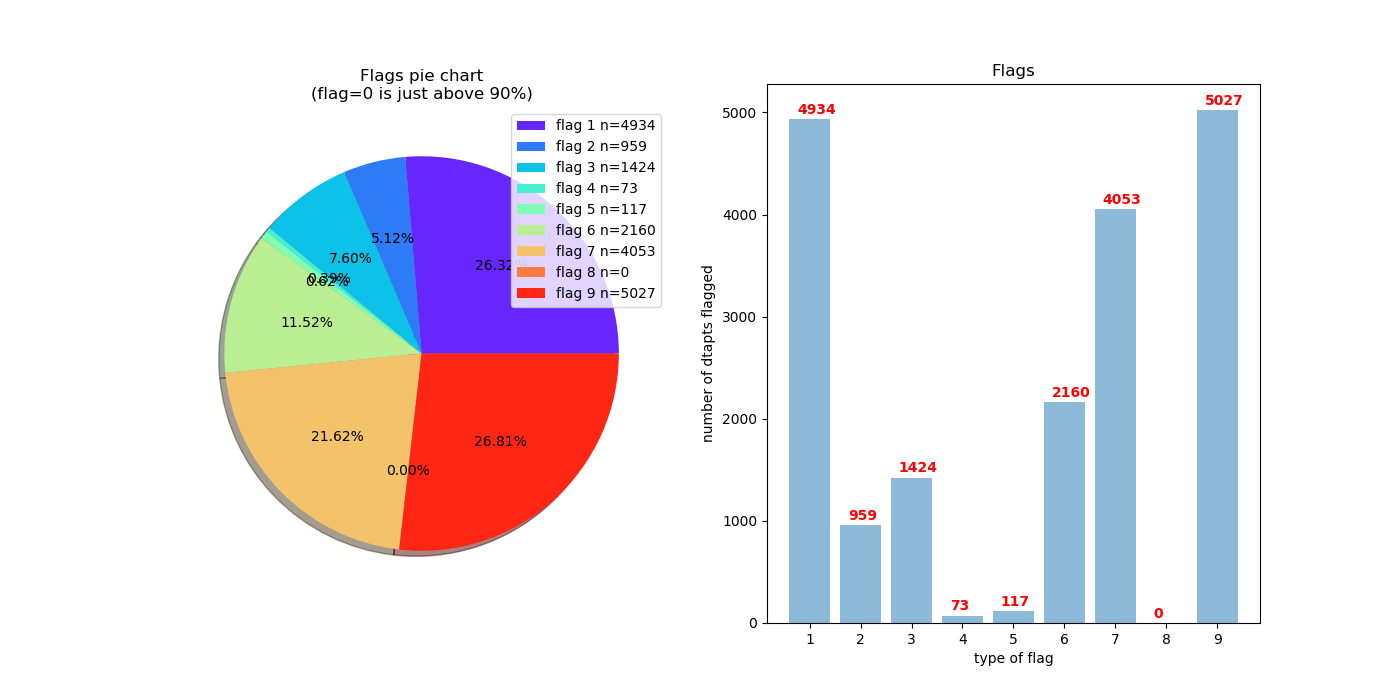
\includegraphics[width=\linewidth]{pie-charts-3-flags.png}
\par}


\section{Modifications made to the database}\label{section:modifications made}

{\centering
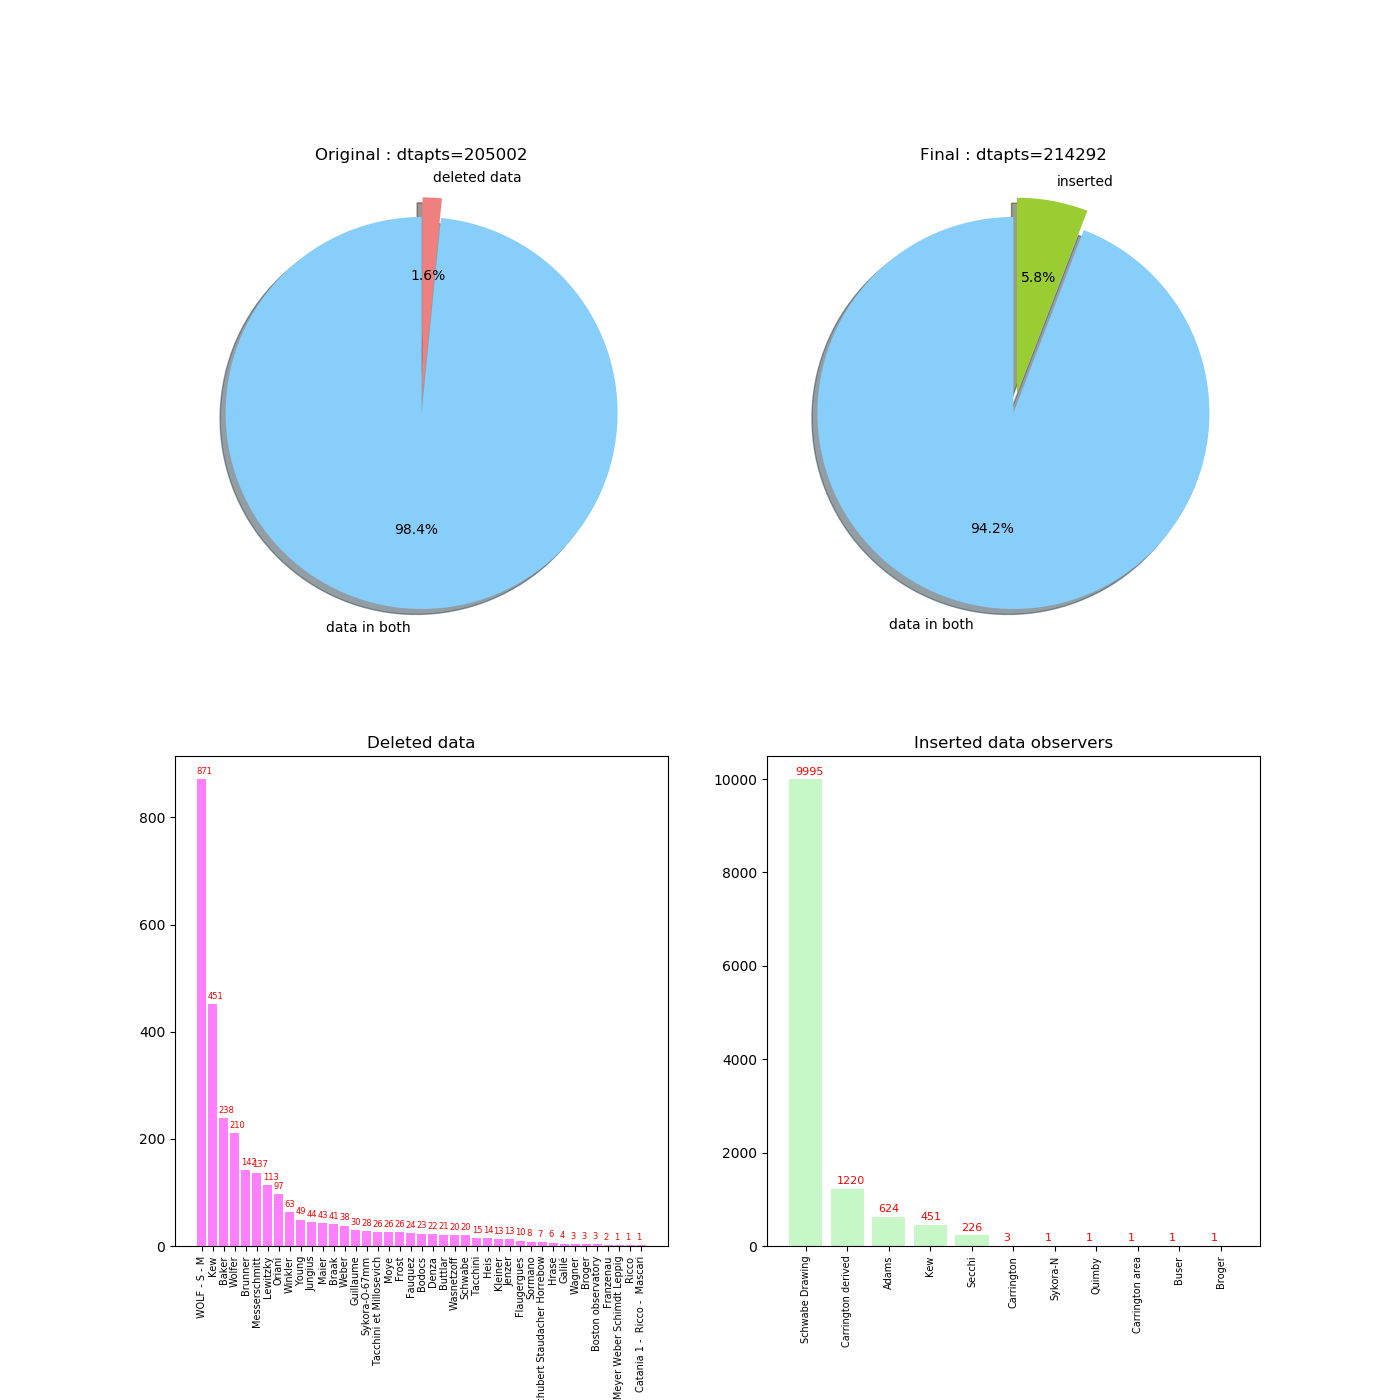
\includegraphics[width=\linewidth]{pie-charts-1-deleted-inserted.png}
\caption{Number of data-pts deleted or inserted}
\label{fig:pie chart deleted inserted}
\par}

{\centering
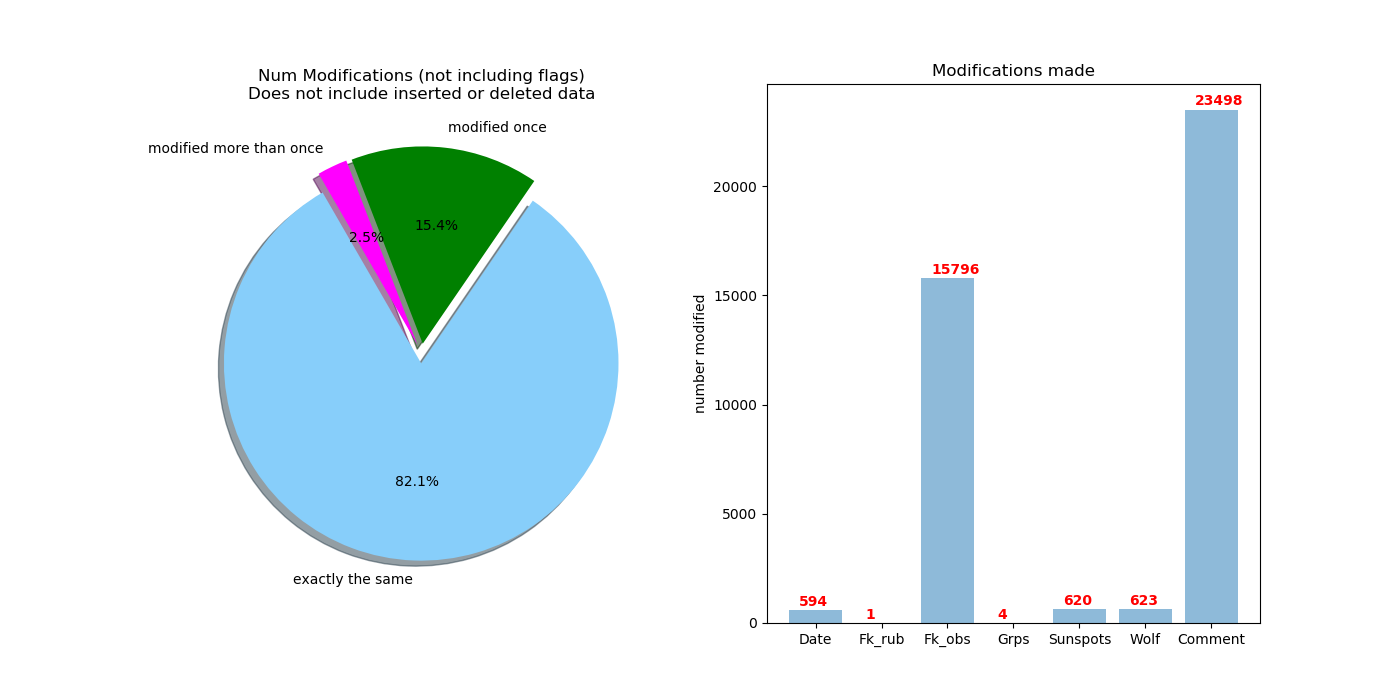
\includegraphics[width=\linewidth]{pie-charts-2-modified-database.png}
\caption{Data that was modified}
\label{fig:pie chart modified data}
\par}

For further information on the issues presented by each of these flags see section \ref{section:issues with flags}

\subsection{Duplicated data}\label{section:duplicated data}

This is the data for which a single observer has more than one data-point associated with him on a single day, there were roughly 14000 of these. A fuller description of the types of duplicated data can be found in the duplicates folder - in particular \href{https://github.com/dcxSt/DATA_SILSO_HISTO_search/blob/master/duplicates/3\%202019.06.27/corrections_needed_handwritten.md}{this file}. The following is an outline of the types of duplicate data and what I did with them. (see June 25++ in log)

\begin{itemize}
    \item[\textbf{Identical}] There were some identical data point, that is to say that the fields \{groups, sunspots, date, wolf, comment, fk\_rubrics, fk\_observers\} were exactly the same for several data-pts. Here I deleted all but one.
    \item[\textbf{!Year}] There were entire rubrics where all the fields were entered in correctly except for the year, these ones were easy to correct because the rubrics id gave them away.
    \item[\textbf{!Obs}] Like with the incorrect year entire rubrics where entered in correctly except for the observer, they were also corrected.
    \item[\textbf{$2^{nd}$ Obs}] There were cases (notably Brunner and his assistant), where several observers share the same observation table and some of their observation days overlap. These observers where separated out. 
    \item[\textbf{!Alias}] Some data was entered twice under several different observer id number, but where the two id numbers were associated with the same alias.
\end{itemize}


\subsection{Sorting comments}\\

I arranged all the comments into sections according to which rubrics they appeared in and sorted them into different types with the following colour code. Some comments are associated with several of the following colours. Originally there were 8043 commented data-points, (there are now 34875 but this part is concerned with the original comments).

\begin{itemize}
    \item[\textbf{Pink}] Several comments which mean the same thing. For instance in rubrics 757 there is 1 data-pt with comment `* = Wolfer P' and 30 data-pts with comment `*'. Nothing else is commented in this rubrics. For these types of comment. Having checked the Mittheilungen to confirm my suspicion I changed the short version of each comment and turned it into the long version, in our example we end up with 31 data-pts with comment `* = Wolfer P'.
    \item[\textbf{Orange}] Commented observer / secondary telescope. Many of the data-pts including the one in the previous example have the real observer commented. In the Mittheilungen journals there are many rubrics where most of the observations are made by one observer, but some are made by another. These rubrics were often typed in under the primary observer only, but with the name of the secondary observer(s) / telescope(s) commented in where indicated in the journals. Often the comments were a single letter. I modified all these comments so that each comment clearly listed either the name of the secondary observer / instrument where indicated.
    \item[\textbf{Red}] There is one type of comment that appears many times in different forms, these are the comments which turned into the flag 2 (see \ref{table:flags key}). The data-points in question are the ones where the comment looks like one of these \{uncertain, Uncertain, ?,  mauvaise def img sol, mauvaise definition image du soleil, bad quality sun image\}
    \item[\textbf{Blue}] Number comments are other strange comments. These are the data-pts where the comment may look like one of these \{0.3 , 0.5 , 2.5 , 1 1 , 14 2 9 , img. 20 cm diameter , 9.5 cm image, derived 29, derived 11\}. The numbers sometimes made reference to a secondary observer who observed on the same day as the primary observer of a rubric; in Secchi's case (derived $n$) the comment indicated the sunspot number derived from his umbra surface area measurements. I modified the data where appropriate.
    \item[\textbf{Other}] There are also those comments I could not classify easily, these ones I looked up individually (as with the blues) and dealt with them on a case by case basis. \ref{fig:carrington kew jenzer leppig sunspots plot} ; \ref{section:derivation from area}
\end{itemize}


\subsection{Separating aliases with several observers.}
There are some observer aliases that contained several names in them. This is an issue because it creates gaps in certain observer's data. The following is a summary of the data where I changed the \texttt{FK\_OBSERVERS} field to deal with this problem. 

\subsubsection{Billwiller et Wolfer}
Rubrics 411 with 256 data-pts containing data from Billwiller and Wolfer under the alias fk=53, alias=`Billwiller et Wolfer'. The data was changed so that the observations were attributed to either `Billwiller' or `Wolfer' (July 18) 

\subsubsection{Wolfer, Mooser }
Rubrics 643 has 297 data-pts containing data from Wolfer and Mooser under alias fk\_obs=122, alias=`Wolfer, Mooser '. The data was changed so that the observations were attributed to either `Wolfer' or `Mooser' (July 19)

\subsubsection{Wolf P-M Wielenmann Mayer Schwabe Weber - fk\_obs=60}
Rubrics fk\_rub=218, it doesn't have a rubrics number (385 dta-pts). It is a table that contains data from the 5 observers listed above. I was able to separate the observations made from this table into separate observers. (see July 22)

\subsubsection{Wolf P-M Meyer Schwabe Weber Schmidt - fk\_obs=61}
fk\_rub=138, no rubrics number (346 dta-pts). The data was sorted in a similarly as with the above. (July 22)

\subsubsection{Wolf P-M Meyer Weber Leppig - fk\_obs=62}
fk\_rub=219, no rub number (339 dta-pts). The data was sorted in a similar way as above. (July 22)

\subsubsection{Ricco, Zona, Mascari - fk\_obs=93}
There were only 8 data-pts associated with this observer alias to start with. The rubrics number is 592 and fk\_rub=371. All 8 of the dta-pts were observed by Ricco, so I modified them appropriately.

\subsubsection{Sykora, Jastremsky}
Rubrics 767, all the data except for 4 dta-pts is Sykora. The remaining 4 were Jastremsky. They were moved to their own observer aliases appropriately. (see August 6) (see section \ref{section:info sykora} for info about the three Sykora's)

\subsubsection{Popow, Sykora-N-6ft}
fk\_observer = 136. This observer is associated with data from both Popow and Sykora-N's observations. The data belonging to Sykora-N was modified appropriatley, however Popow did not have his own alias and all of his observations are in this rubric, so I merely modified observer fk\_obs=136 so that the alias is now `Popow'.

\subsubsection{Tacchini and Milesovich}
In 1881 the rubrics number 465 contains two data sets, one of them is entirely Ricco's and the second is from Tacchini and G. Millosevich. Nowhere in the data set is it indicated who saw what, so I looked and found that there was no Alias for Millosevich. This makes me think that he must be Tacchini's assistant or observing partner. Anyway we have a big gap in Tacchini's observations, what I will do is comment all of these observations `Tacchini and Millosevich'. I did that and gave them a flag=3, there is no more gap in 1881 in Tacchini's graph, what's more the data looks almost identical. 

\subsubsection{Tacchini und G. De Lisa}
Precisely the same thing happens to Tacchini in 1877 and 1878 but this time it is `Tacchini und G. De Lisa'. I did the same as with Milesovich. Flag=3, De Lisa is commented. (See figures at \ref{fig:tacchini display seperate flags all} and \ref{fig:tacchini display seperate flags sunspots})

\subsection{Derivation of wolf number from umbra area measurements}\label{section:derivation from area}\\

By plotting certain observers you can see that there is clearly something wrong with some of the data.\\

{\centering
%\begin{figure} % i gave up on figures, I don't understand them
\caption{Carrington and Kew umbra area measurements in sunspots field \\(see \ref{fig:carrington, kew, leppig, jenzer after fix} for plot of the derived data)}
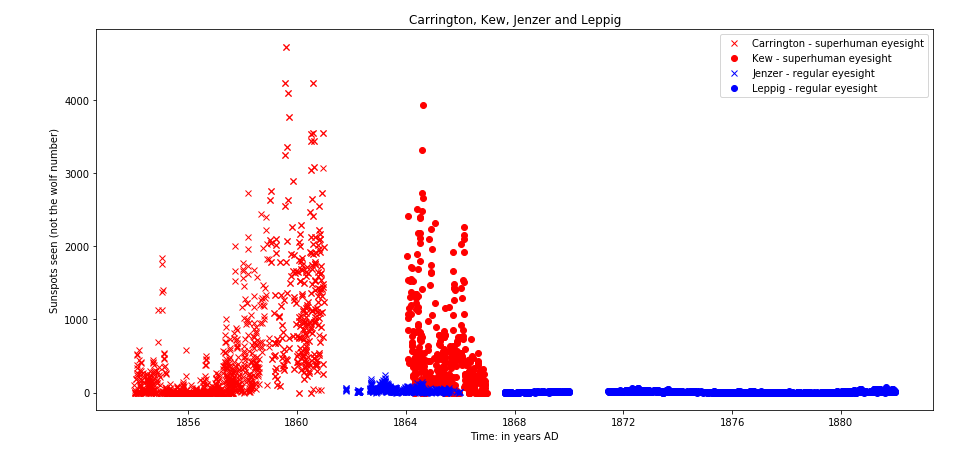
\includegraphics[width=\linewidth]{CarringtonHasGoodEyesight.png}\label{fig:carrington kew jenzer leppig sunspots plot}
%\end{figure}
\par}

\subsubsection{Secchi}
In rubrics 299 the data-table contains Angelo Secchi's group measurements and total area of the sun disk covered by umbra of the sunspots measurements, along-side sunspot number estimates $s$ that he derives $s = f \cdot 0.15$. The factor of 0.15 he derives by least-squares fit. The assumption he makes is that the wolf number $r$ is related to the groups number $g$ and the area measurement $f$ as described by equation \ref{equation:derivde wolf}
$$
r = a \cdot (10 g + b\cdot f)\quad \text{ with } a,b\in\R
$$
He obtained the values $a = 1.41\quad b=0.15$ by doing a least-squares fit. $\chi^2$ is given in equation \ref{equation:chi-squared}. I used the data Wolf had derived in the comments for the sunspot number.\\

Below is a scatter plot of Secchi's data. As you can there are still problems with it. from mid 1873 we only have data for the number of groups observed, and in 1872 there is a hole in the data.\\

%\newpage
{\centering
    %\caption{Secchi's data seperated by flag; wolf, sunspots, groups}
    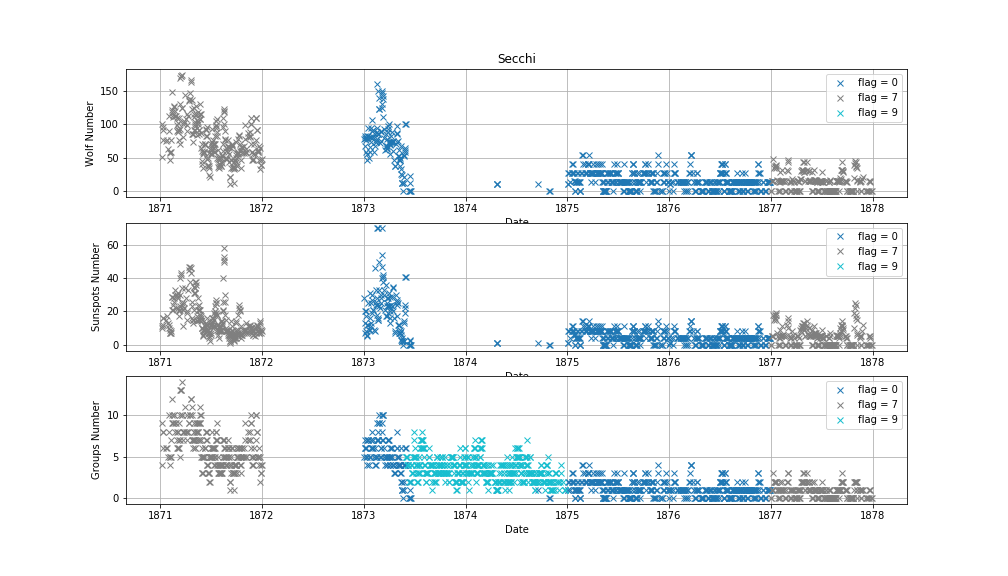
\includegraphics[width=\linewidth]{secchi_seperate_flags.png}
\par}

\subsubsection{Carrington}
Carrington has 7 years worth of observations recorded in the Mittheiulungen journals. For all 7 years he records measurements of the total area of the sun disk that is covered by the umbra of the sunspots as well as the groups number. In 1859 and 1860 Carrington \textit{also} has a table with measurements of the groups and sunspots, it is from this 2 year over-lapping period between the two data-sets that I was able to deduce the value of the parameters $a$ and $b$ for the relationship describe by the author of Rubrics 299. Using equations (\ref{equation:wolf probability}), (\ref{equation:wolf total probability}), (\ref{equation:chi-squared}) and (\ref{equation:chi squared condition for best fit params}). In this case equation \ref{equation:chi squared condition for best fit params} is merely a (long) quadratic equation. I used \texttt{scipy.optimize.curve\_fit} to do this calculation. \\

You may notice a slight hypocrisy - after using an invariant standard deviation to calculate Carrington's best fit parameters, I then display the standard deviation as a percentage of the wolf value. With hindsight I think a more appropriate model for the standard deviation is one which varies with the wolf number $r$ like so $\sigma(r) = \alpha + \beta r$. That said it would have been tricky to implement and perhaps beyond the scope of what is expected. \\

{\centering
\caption{Carrington least squares line of best fit}
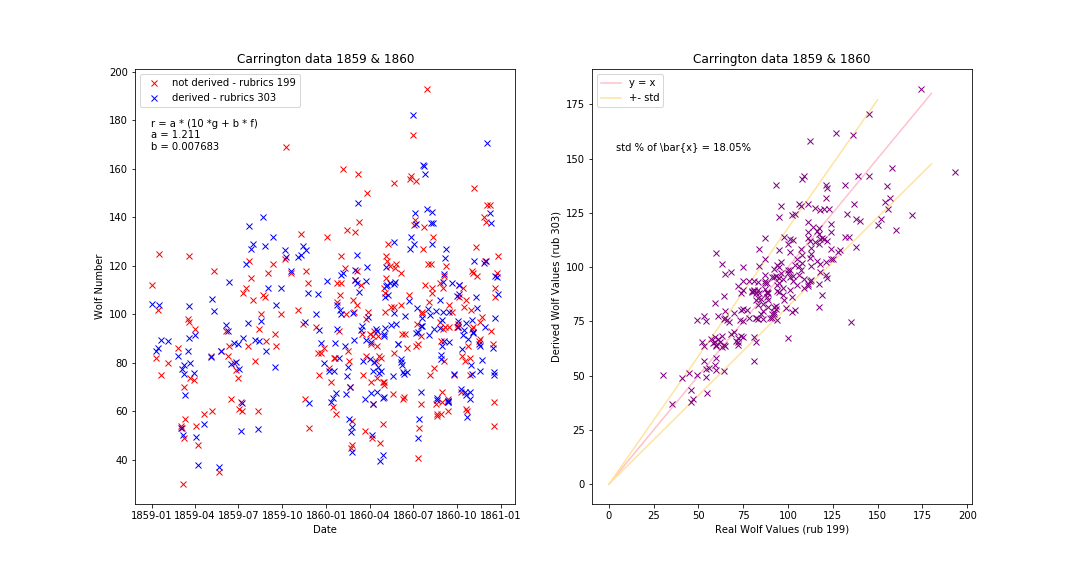
\includegraphics[width=\linewidth]{carrington_fit_wolf.png}
\label{figure:carrington fit wolf}
\par}\\

Carrington's data now resides in 3 seperate observer aliases.
\begin{itemize}
    \item `Carrington' - this is rubrics 199, the data from 1859 and 1860 where Carrington actually recorded the sunspots and groups number.
    \item `Carrington area' - rubrics 303, 7 years worth of umbra area measurements
    \item `Carrington derived' - rubrics 303 transformed by equation (\ref{equation:derivde wolf}) using the best fit parameters $a=1.21$ $b=0.00768$
\end{itemize}

\newpage

{\centering
    \caption{Carrington's derived data}
    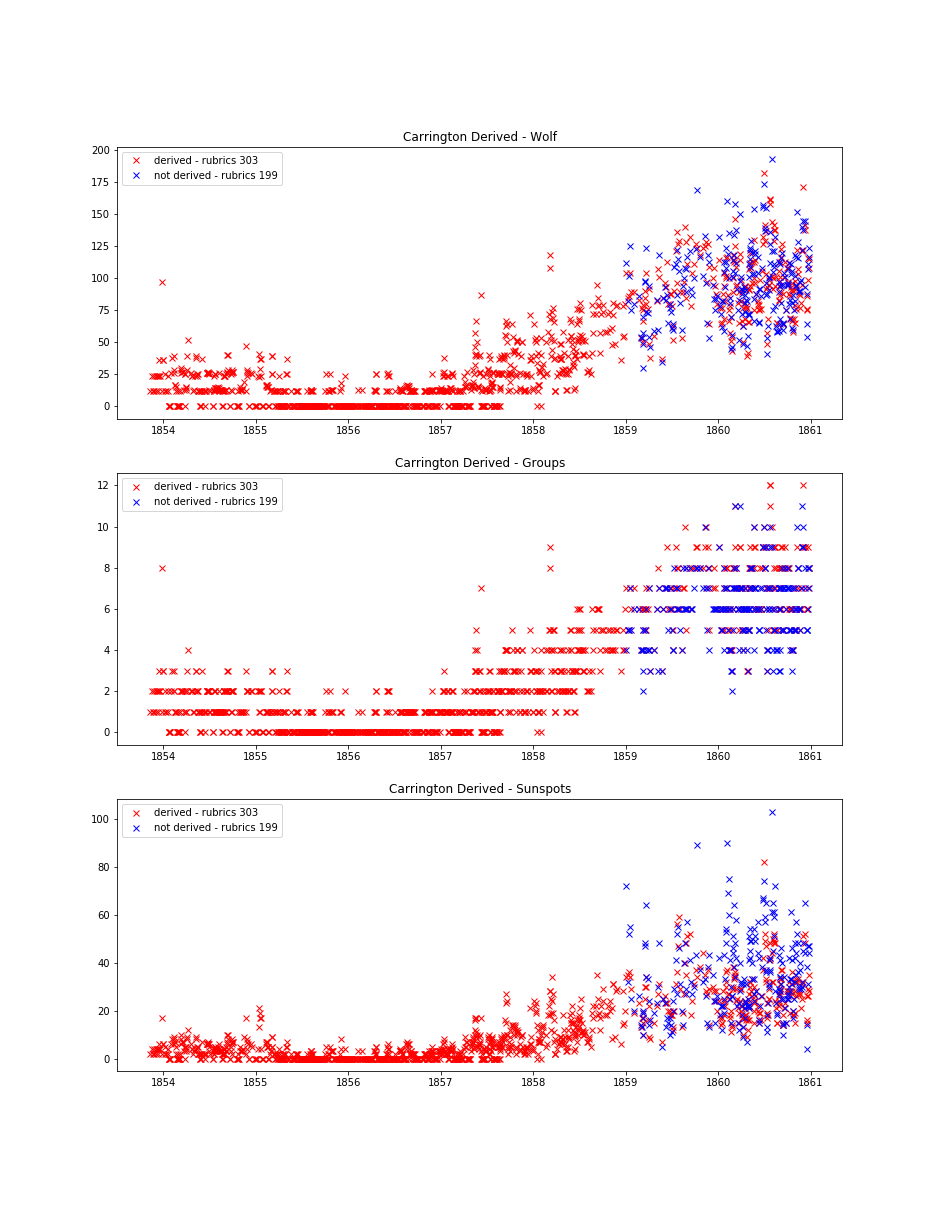
\includegraphics[width=0.9\linewidth]{carrington_derived.png}
    \label{figure:carrington derived}
\par}

For further detail on Carrington and Secchi see July 5 to 10 in the log. Further I translated Rubrics 299 with \href{https://www.deepl.com/translator}{deepl.com/translator} - an online translator, the rubrics (in English and German) can be found in section 5 of the log.

\subsubsection{Kew}

Applied the same fix to Kew that I did to Carrington. In Kew's case the Mittheilungen did not have any sunspots / wolf number data - only groups and total umbra area of sun-disk. The good news is that the author of rubrics 306 already did the work for me and has found $a = 0.763$, $c = 0.032$ $\RA b = 0.042$
$$r' = 0.763 \cdot (10 g + 0.042 f)$$

Here is a plot of Carrington, Kew, Jenzer and Leppig's data similar to the one above but this time using the values transformed by Wolf's umbra conversion formula. Which looks much more like it should.\\

\\
{\centering
\caption{Carrington and Kew derived measurements (see fig \ref{fig:carrington kew jenzer leppig sunspots plot})\\using display compare observers method}
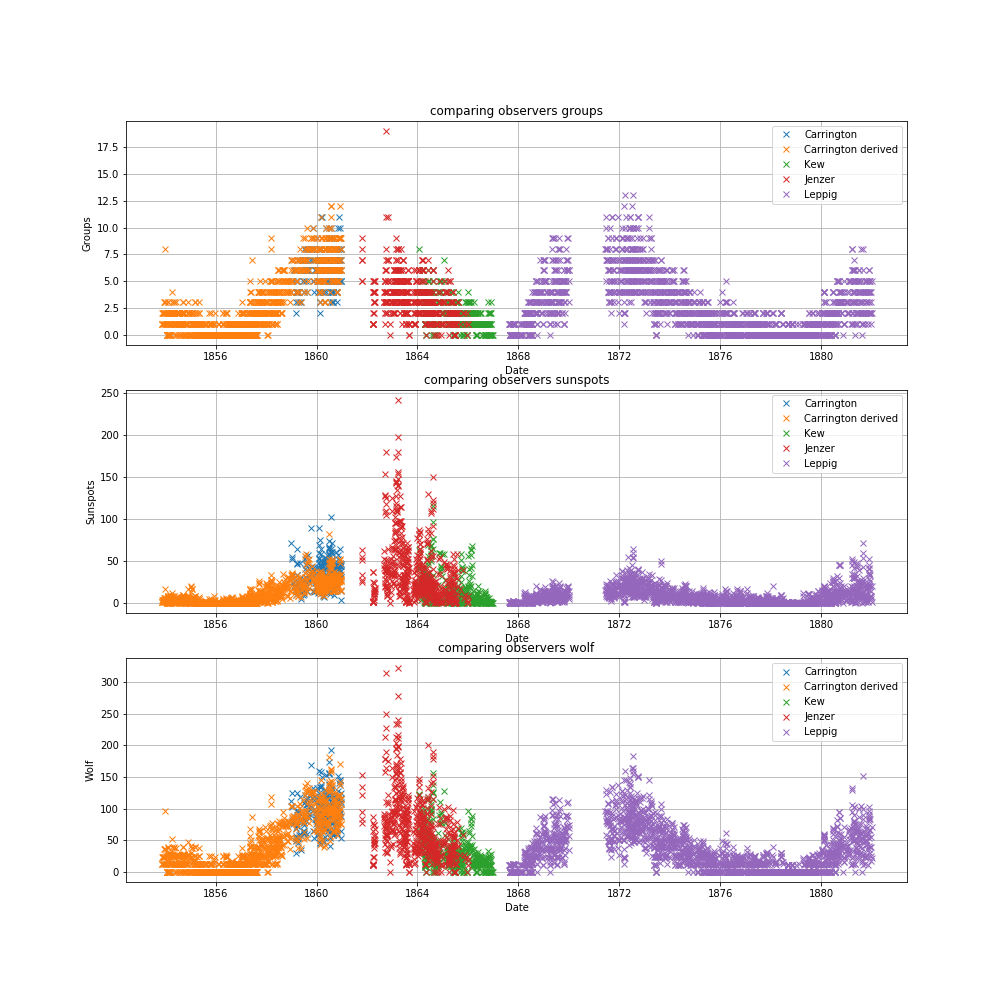
\includegraphics[width=\linewidth]{carrington_kew_after_fix.png}
\label{fig:carrington, kew, leppig, jenzer after fix}
\par}


\subsection{Inserting Schwabe's diagram data}
Motivation / Why outline the process of insertion? This is important because it is just possible that it's not exactly right. \href{https://www.aip.de/Members/rarlt/sunspots/schwabe}{Source of Schwabe's online data} The actual data I incorporated into the base was from \texttt{schwabe\_v1.3\_20150812.txt}\\

According to modern understanding some groups were split and some were merged. Where it is written 126-0, this means there is a 126-1. Schwabe saw one group we see two. When it says 303+304 this means groups 303 and 304 as seen by Schwabe are in-fact the same group. Consequentially `Schwabe Drawing' and `Schwabe' are two very different observers, they will have a different finger-print of observational bias.\\

The text file with the online data can be found in the folder `data\_other\_sources/' in the project's root directory. The columns we are interested in are \\

{\centering
\begin{tabular}{c|c|c|c}
    YYYY & MM & DD & GROUP 
\end{tabular}
\par}\\

The data contains much more information than we need. For each day of observation, there is one entry for each sunspot, the entry specifies which group the sunspot belongs to in the GROUP column, and where on the sun it is at what exact time of day with what area of umbra etc. So the number of entries each day is the number of sunspots, and the number of different groups (they are classified by group id) is the number of groups. The wolf number was calculated with the usual formula $r = 10g + s$. See jupiter notebook \texttt{Schwabe Drawings data.ipynb} for more information on how the calculation was made. \\

{\centering
\caption{Schwabe Drawing Figure}
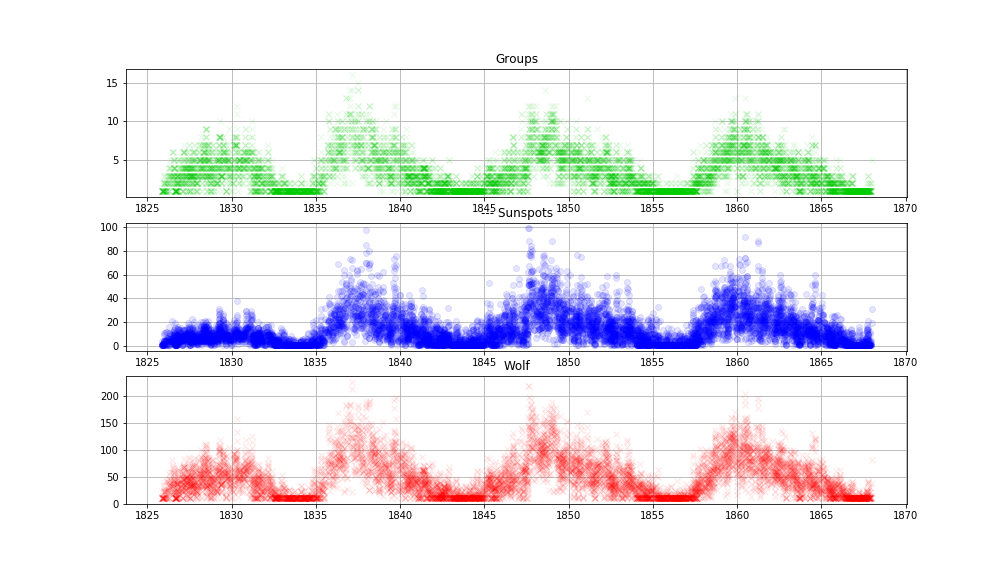
\includegraphics[width=\linewidth]{Schwabe-Drawing.png}
\label{fig:schwabe drawing}
\par}


\subsection{Kremsmunster observatory}
There is confusion about the observer, a little investigation was conducted online and I uncovered some useful information about who was observing at the observatory, but not enough to deduce exactly who to attribute the observations to. The data is a bit of a mess :(. The troublesome data can be found in rubrics 684, mitt 83, pages 97-106 (it's a big rubric spanning several years). To give a brief outline of what is wrong : there is ambiguity as to whom the observer is, the observations therefore are attributed to aliases relating to Kremsmunster ; there is also the problem that there several different telescopes are used and several methods of counting sunspots are used - there are two main telescopes (Achromaten \& Theodolitfernrohr), and the sunspots number is sometimes recorded by the observers, and sometimes they are deduced using modern methods from a sketch of the solar disk. (see July 25 / 26 in the log).\\

{\centering
%\caption{Before and after}
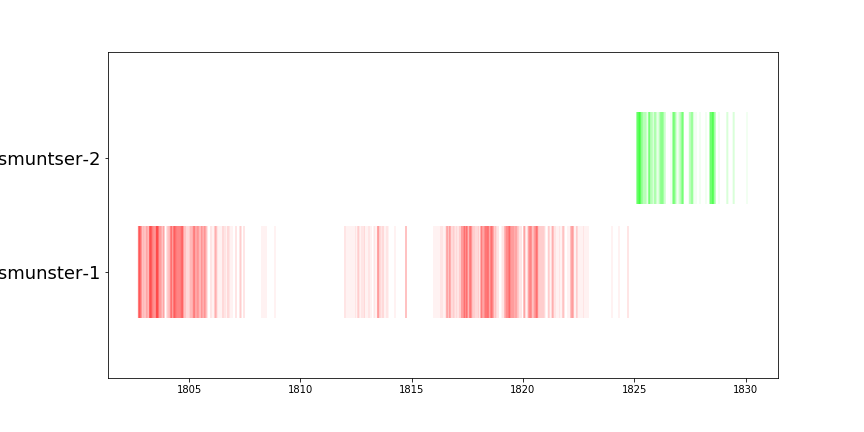
\includegraphics[width=0.49\linewidth]{kremsmunster_event_og.png}
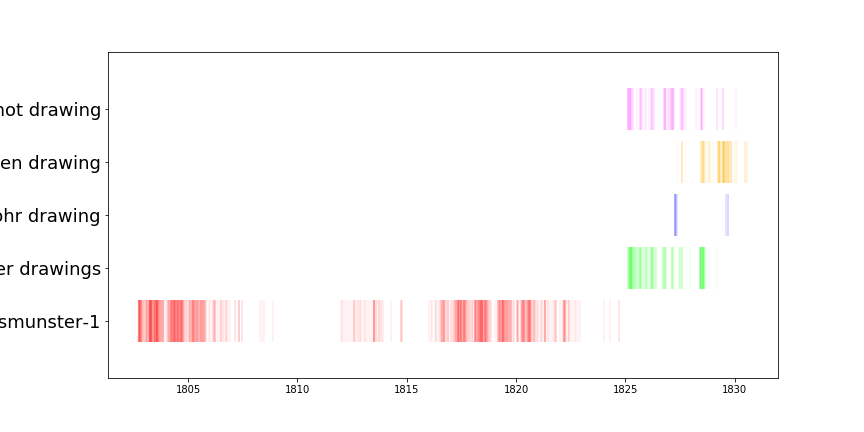
\includegraphics[width=0.49\linewidth]{kremsmunster_event_after.png}
\par}

{\centering
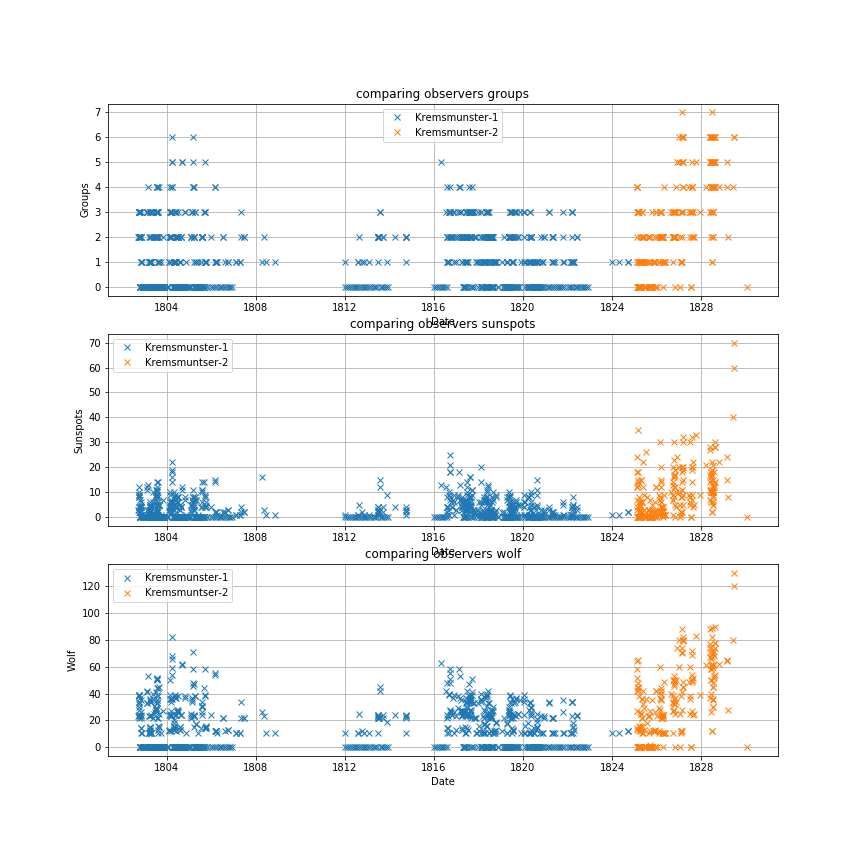
\includegraphics[width=0.49\linewidth]{kremsmunster_scatter_og.png}
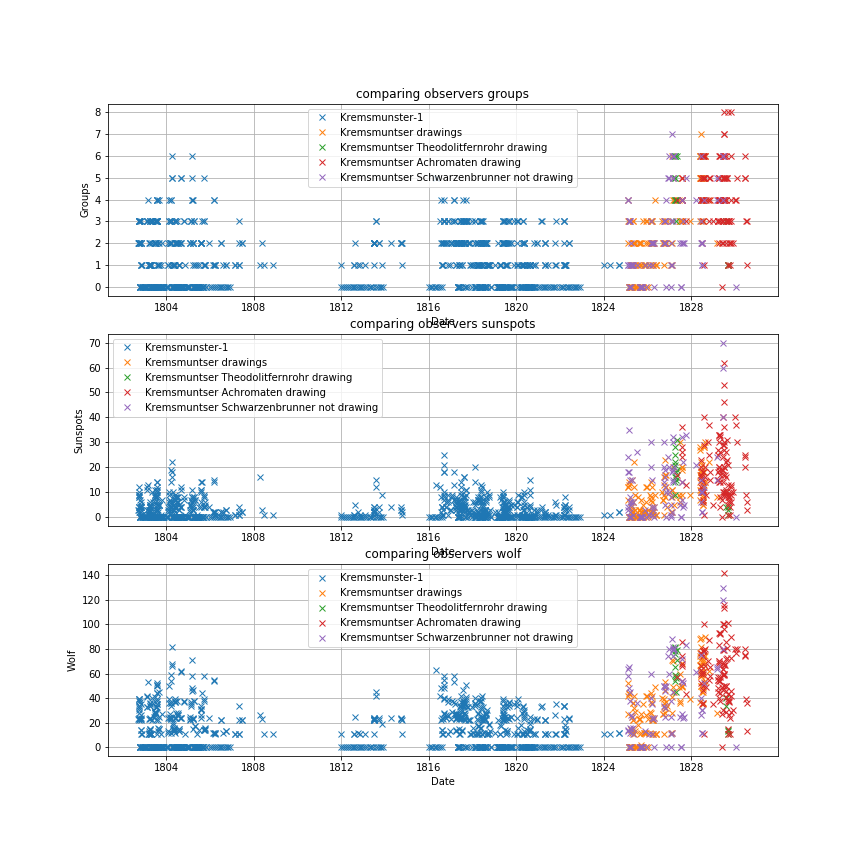
\includegraphics[width=0.49\linewidth]{kremsmunster_scatter_after.png}
\par}\\

\subsection{Other corrections}

\subsubsection{Adams}
In rubrics 167 there are periods where it is written `None observed' from this date to that date in the Mittheilungen (Jul 17). I entered these in the data-base as 0.0 data-points and commented them `None visible', with no flag. I think these periods contain data with 0.0 rather than being days that Adams did not observe the sun are for reasons (a) and (b); for reason (c) it is important that they are included and not neglected.
\begin{enumerate}[(\alph*)]
    \item On the days that observers don't observe there is no data rather than a `none visible' from this date to that date comment
    \item There are long periods where there is no Adams data in the same table, so why would Adams sometimes put None visible and then sometimes just put nothing.
    \item It is important to include dates where Adams observed no activity in the database or his monthly / yearly averages will be completely skewed, specially because this is during a minimum.
\end{enumerate}

\subsubsection{Miscellaneous}
\begin{itemize}
    \item Numerous typos were found along the way, these were corrected individually.
    \item Rubrics 828 - changed the observer from `Konkoly' to `Scharbe', and where there was P commented, the observer became `Pokrosky'
    
    \item Some data from `Schwab' had been attributed to `Schwabe' - these are two different people that lived in different centuries. (Jul 16)
    \item Stempel observerd in two different ways.
\end{itemize}


\section{Herr R.Wolf and Herr Wolfer - controversial transition period}

\subsection{Wolf}
Table of each of Wolf's rubrics and which telescope he uses from 1870 on-wards. The motivation for this is that after learning about how much of a hotly disputed topic Wolf was I though it was a good idea to really present Wolf's data in as clear a manner as possible.\\

KEY\\
\begin{itemize}[\ddagger]
    \item Quadruped = \textit{` der entweder von mir oder von Herrn Meyer nach ganz entsprechender Art mit Vergrosserung 64 meines Vierfussers erhaltenen Normalbeobachtungen'} $\longrightarrow$ \textit{normal observations received either from me or from Mr. Meyer in quite appropriate way with enlargement $\times 64$ of my four-footer}
    \item $2\frac{1}{2}$ foot = \textit{` einem 2 1/2 Fusser bei Vergrosserung $\times 42$ gemacht'} $\longrightarrow$ \textit{a 2 1/2 ft made with enlargement $\times 42$}
    \item Parisian = \textit{` $2\frac{1}{2}$ füssigen Pariser-Fernrohr bei Vergrösserung 20 gemacht'} $\longrightarrow$ \textit{the $2\frac{1}{2}$ foot Parisian telescope with enlargement factor $\times 20$}
    \item Parisian$\dagger$ = Most probably the Parisian telescope : \textit{` Ein beigesetztes * bezeichnet Beobachtungen, welche ich mit dem kleinern Instrument machte, und mit 3/2 in Rechnung brachte '} $\longrightarrow$ \textit{A * indicates observations, which I made with the smaller instrument, and charged with 3/2.}
    \item Pocket 1 = \textit{`wenigen mit * bezeichneten Beobachtungen wurden auf Ausflugen mit einem kleinen Taschenfernrohr erhalten'} $\longrightarrow$ \textit{observations marked with * were obtained on trips with a small pocket telescope}
    \item Pocket 2 = \textit{`Die mit * bezeichneten Beobachtungen sind auf Ausflugen mit einem kleinen Taschenfernrohr angestellt, und werden mittelset des Factors $\frac{3}{2}$ den übrigen homogen gemacht'} $\longrightarrow$ \textit{observations marked * are made on excursions with a pocket telescope, the observations are homogenised by means of a $\frac{3}{2}$ adjustment factor}
    \item A telescope in brackets e.g. (Parisian) means that \textbf{no telescope was mentioned} but what is in the brackets is almost certainly the one used.
    \item Wolf + Carr = I could not find a description of the telescopes used by Wolf or Carrington, he just says somewhat cryptically that the unmarked observations were made by him and Carrington
    \item s = observations made by Schwabe that found their way here
    \item var = various observers, a whole host, usually 4 or 5. 
\end{itemize}


{\centering
    \begin{tabular}{c|c|c|c|c|c|c|c}
        Rub_{id} & Rub_{no} & Mitt no & Page & Date & Primary & *=Secondary& Comments \\
        \hline
        - & 0 & 1 & 153-9 & 1849-55 & var & - & see footnote \footnotemark[7] \\ 
        - & 0 & 3 & 110 & 1856 & var & - & - \\ 
        - & 0 & 6 & 125 & 1857 & var & - & - \\
        - & 0 & 8 & 67 & 1858 & var & - & - \\
        - & 0 & 11 & 2 & 1859 & Wolf, Carr, s & - & see footnote \footnotemark[6] \\
        - & 0 & 12 & 69 & 1860 & Wolf + Carr & Parisian$\dagger$ + s & mostly primary \footnotemark[5]  \\ 
        - & 0 & 14 & 120 & 1861 & $2\frac{1}{2}$ foot & Parisian$\dagger$ & primary obs = Wolf\\
        &&&&&&& mostly secondary\\
        - & 0 & 15 & 134 & 1862 & Quadruped & Parisian$\dagger$ & primary obs = Wolf\\
        &&&&&&& mostly secondary\\
        - & 0 & 16 & 164 & 1863 & Quadruped & Parisian$\dagger$ & primary obs = Wolf\\
        &&&&&&& mostly secondary\\
        - & 0 & 17 & 194 & 1864 & Quadruped & Parisian$\dagger$ & primary = Weilenmann + Wolf \\
        &&&&&&& mostly secondary till winter\\
        - & 0 & 21-30 & 18 & 1865 & Quadruped & Parisian$\dagger$ & prim: Weilenmann, Fretz, Wolf \\
        &&&&&&& mostly primary\\
        - & 0 & 21-30 & 74 & 1866 & Quadruped & Parisian$\dagger$ & prim: Weilenmann, Fretz, Wolf \\
        &&&&&&& mostly primary\\
        218 & 0 & 24 & 104 & 1867 & Quadruped & Parisian$\dagger$ & prim: Weilenmann, Meyer, Wolf \\
        &&&&&&& roughly half half\\
        219 & 0 & 26 & 208 & 1869 & Quadruped & Parisian$\dagger$ & primary: Meyer + Wolf\\
        158 & 274 & 30 & 403 & 1870-71 & Parisian & Pocket 1 & Mostly primary \\
        165 & 289 & 33 & 111 & 1872 & (Parisian) & Pocket 2 & Mostly primary \footnotemark[4] \\
        179 & 313 & 36 & 266 & 1873 & (Parisian) & - & 100\% primary \\
        186 & 326 & 38 & 394 & 1874 & (Parisian) & - & 100\% primary \\
        192 & 335 & 39 & 418 & 1875 & (Parisian) & - & 100\% primary \\
        198 & 344 & 42 & 50 & 1876 & (Parisian) & - & 100\% primary \\
        205 & 365 & 46 & 185 & 1877 & (Parisian) & - & 100\% primary \\
        212 & 385 & 49 & 251 & 1878 & (Parisian) & - & 100\% primary \\
        236 & 410 & 50 & 298 & 1879 & (Parisian) & - & 100\% primary \\
        220 & 430 & 52 & 50 & 1880 & (Parisian) & - & 100\% primary \\
        258 & 453 & 55 & 160 & 1881 & (Parisian) & - & 100\% primary \\
        288 & 470 & 59 & 337 & 1882 & (Parisian) & - & 100\% primary \\
        247 & 488 & 62 & 84 & 1883 & (Parisian) & - & 100\% primary \\
        266 & 505 & 64 & 158 & 1884 & (Parisian) & - & 100\% primary \\
        281 & 522 & 67 & 299 & 1885 & (Parisian) & - & 100\% primary \\
        295 & 539 & 69 & 349 & 1886 & (Parisian) & - & 100\% primary \\
        329 & 563 & 71 & 16 & 1887 & (Parisian) & - & 100\% primary \\
        358 & 584 & 73 & 109 & 1888 & (Parisian) & - & 100\% primary \\
        386 & 603 & 76 & 226 & 1889 & (Parisian) & - & 100\% primary \\
        418 & 624 & 78 & 296 & 1890 & (Parisian) & - & 100\% primary \\
        433 & 642 & 80 & 381 & 1891 & (Parisian) & - & 100\% primary \\
        312 & 664 & 82 & 53 & 1892 & (Parisian) & - & 100\% primary \\
        330 & 685 & 84 & 120 & 1893 & (Parisian) & - & 100\% primary \\
        
    \end{tabular}
    
    \label{table:silly table version 2}
\par}\\

% use footnotes from 4 and onwards
\footnotetext[7]{For more information on rubrics 1 which contains a huge chunk of WOLF - S - M from 1849-55 see \ref{mitt:rub 1}}
\footnotetext[6]{As indicated the observers are all mixed up, however he does specify outside the table the days where Schwabe is the real observer. This data seems to have been correctly digitized.}\\
\footnotetext[5]{This year he uses His and Carrington's data from 1859 and 1860 to derive the correction factor $k=1.5$ for his Parisian telescope, and also for Schwabe but this is less important. Further, he finds that Carrington's k factor is the same as his.}\\
\footnotetext[4]{\textit{Pocket 1} and \textit{Pocket 2} are the same telescope, but only for \textit{Pocket 1} is there mention of a correction factor}\\

\\

Conclusions:
\begin{itemize}
    \item Things look very good for WOLF - P - M, asides a handful of observations in 1870-72 all the data seems to have been entered in correctly. Everything after 1872 is almost definitely correct (ignoring the fact that there may be typos). Before 1870 it's slightly trickier, I still haven't excluded the possibility that Wolf may have been using the Pariser as far back as the 1850's but just failed to mention it. 
    \item As for WOLF - S - M things are not so good. From 1849 to 1860 we have no way of identifying which observations are Wolf's own, let alone what telescope he was using. The only information he provides us with from 1856 on-wards is how many days of the year he observed, and how many days he used other people observations, but not exactly when - actually he doesn't even tell us that, he says how many days he or his assistants observed though the quadruped $\times 64$ magnification telescope.
    \item There are 526 flag = 1 observations with WOLF (S-M \& P-M) as observer. 36 of these are because they are not his, I haven't moved them because I haven't yet found out whose they are (the observations are attributed to Wolf before 1849). Most of the others seem to have missing sunspots numbers, some of them are marked as having missing groups but I suspect the digitizer just typed the group number into the sunspots column because most of these are $x\leq 5$. These still have to be dealt with. This may involve deriving a formula that guesses a wolf number based purely on the group - perhaps it could also take as a parameter what the average sunspot index is (heavily smoothed) around that time, but I shouldn't get ahead of myself I still have alot to do and not much time.
       \item List of key dates given by F. Clette 2019/08/06.
    \begin{itemize}
        \item[$\bold{1849}$:] Schwabe Wolf
        \item[$\bold{1861}$:] introduction of $k$ factor and Wolf starts to use other observers' observations (alongside his own)
        \item[$\bold{1864}$:] Opening of the Zurich Observatory and hiring of his first assistant
        \item[$\bold{1877 / 78}$:] Arrival of Wolfer
    \end{itemize}

\end{itemize}

\subsection{Wolf log}
\begin{itemize}
     \item[\textbf{1856:}] One table entered into `WOLF - S - M' that has data gathered by Schwabe but it is uncertain as to which points exactly are his. \textit{The stars in the table are to indicate the appearance of new sunspot groups.}
    
     \item[\textbf{1857:}] Just like 1858 - Mitt 7?, Rub 0, page 125. \textit{Same as above.} 
    \item[\textbf{1858:}] Mitt 1, Rub 0, page 67. There is only one table entered into `WOLF - S - M', it has in it some data gathered by Schwabe. There is no sign of there being any rubrics associated to Schwabe
    
 \item[\textbf{1859:}] There seem to be holes in WOLF - S - M where there is data in Schwabe, I think we only have Schwabe's data from when Wolf thought it was important.
    \item Mitt XXX and Mitt XXVIII (see the relevant rubrics in the log, the pertinent information is translated.)
    \item I'm checking now to see if there is any data from WOLF - S - M hiding in WOLF - P - M after the year 1870.
    \item I fear Wolf uses 3 telescopes... `observations with enlargement 64 of my quadruped [...] enlargement 64 of my quadruped normal observations (1868) [...] with enlargement of 64 of my four-foot (1869)' ; `$1 \frac{1}{2}$ foot Parisian telescope at magnification 20 (1870 & 1871 - rub 274) [...] dafuer gebrauchten $2\frac{1}{2}$ fuessigen Pariser-Fernrohr (1872, 1873, 1874 - rub 289, 313, 326) [...] ' ; * = `a small pocket telescope' always. The years after 1874 I will take on trust that the observations are all made with the Parisien-fernhohre. The situation we face now is that Wolf suddenly changes his primary telescope at the start of 1870, and that none of the data after 1870 is sorted correctly into primary secondary. Before creating a new observer alias and re-sorting all the data we must first be sure of this. It seems suspicious to me that the change in telescope coincides perfectly with the new year...
    \item There are some strange things going on with Mitt 28 and 30: In the table at the beginning of Mitt 28 there is data taken from the observatory with the big telescope - the quadruped with $\times 64$ magnification, but the majority of the observations in this table are marked with an asterix *, they are referred to as `Ein beigesetztes * bezeichnet Beobachtungen welche ich mit dem kleinern Instrumente machte und mit $\frac{3}{2}$ in Rechnung brachte' ; In Mitt 30 rubric 274) we find a table where the overwhelming majority of the measurements are made with the Parisian telescope `Die grosse Mehrzahl der Beobachtungen ist mit dem ofterwahnten $2\frac{1}{2}$ füssigen Pariser-Fernrohr'. If you compare the tables it is evident from the fact that the entire rubric 274 is contained int he Mitt XXVIII table where the * appears. 
    \item The measurements in the Mitt XXVIII table without any markings were made by `von mir oder von Herrn Meyer' with the $\times 64$ quadruped telescope at the Zürich observatory. This seems to be a time where Wolf is retiring and isn't as mobile...
    \item A complication has arrisen by the fact that he referes in the introduction of Mitt 30 to his Parisian telescope as `dem kleinern Instrumente machte und mit $\frac{3}{2}$ in Rechnung brachte'. This means we have not only to separate out Wolf's post 1870 data into `Parisian' and `portable' telescopes, but we also have to check all of Wolf's pre-1870s data to see if the secondary telescope mentioned is the portable one or the Parisian. [We know he's talking about the Parisian in the quote because the observations coincide with those of rubric 274, and because the Parisian also has a correction factor of $\frac{3}{2}$ -- `Vergleichnung $1\frac{1}{2}$' - Mitt XXX, he then uses 1.5 as the correction factor (k factor) for the Parisian in his derivation of the correction factor of his pocket-telescope, and his pocket telescope has a correction factor of 0.56]
    \item[\textbf{1864:}] This year is a big mess:
    \begin{itemize}[$\longrightarrow$]
        \item In the digital database, all data belonging to either WOLF - S - M or WOLF - P - M allegedly comes from rubrics 0. In Mitt 11 to 20 there is a table with WOLF entries, I think this is where it comes from as this table is \textit{not} under any specific rubrics number; it features on the second page of a Mitteilungen journal, before the numbered rubrics start.
        \item The digital database counts 493 WOLF observations for that year, 140 WOLF - P - M (which seems about what you would expect from the table) and 353 WOLF - S - M, which is not only pretty much impossible (the weather isn't that good in Zurich that you have a clear sky 353 days in a year) and doesn't make any sense. What appears to have happened is that the entire table was entered twice into the database, once correctly and once attributing every observation to WOLF - S - M. 
        \item I verified that all the other observers had been entered in correctly (Weber, Jenzer & Schwabe): Jenzer has his own rubric (`Litt. 211') ; Wolf tells us in the text that Weber's data is in rubrics 210 (`Litt. 210') but this time he is wrong, in rubrics 210 there is Heis' data from Münster, not `Weber in Peckeloh', the digital data contains 16 data-points from Weber in this year which matches what is in wolf's table ; the same goes for Schwabe (seemingly entered correctly) only here Wolf doesn't even mention a Schwabe rubrics, he only provides his name in the key to indicated that the observations marked with a \dag\ are from him.
        \item As for WOLF - S - M's data, all the data-points that do not belong to him should be gotten rid of. I tried to do this through the terminal but ran into some problems, so I moved them into the bin using my method \texttt{db\_transfers.move\_wolf\_1864\_to\_rubbish()} and then manually get rid of Jenzer's stuff data-point by data-point, (there were only 4)
   \end{itemize}
    \item The reason I haven't yet deleted R. Wolf's before 1847 data is because I want to find where it comes from... it is already flagged (flag = 1).
       \item[\textbf{1865:}] There is 0 data from either Wolf p or Schwabe. The data for WOLF - S - M is in rubrics 0 -- The data comes from a data-table on page 18 of Mitt 21-30 which features 5 observers: WOLF - S - M (all of his data is here) ; WOLF - P - M (all of his data is here) ; Weber (wolf claims the rest of his data is in Nr. 225 der Litt. but this is false, this is where Heis' data is) ; Jenzer (the rest of his data is in rub 226) ; Schwabe (who doesn't seem to have any data appart from what is on this table). The only thing I can do really is separate them one by one. 
    \item Schwabe's data is mostly missing, all the Schwabe data we have in 63,65,66 etc. are not in the Mitteilungen, there is only a small fraction of Schwabe's data that Wolf included in the introductory tables to fill the gaps where his data was missing. 
    \item Laure showed me of Schwabe's drawing which you can find \href{https://www.aip.de/Members/rarlt/sunspots/schwabe/paper-schwabe-data}{here} and \href{https://www.aip.de/Members/rarlt/sunspots/schwabe}{here} which have been digitised, the number of times that each group is logged in a day is how many sunspots there are in it and the it has everything I need to fix / add some Schwabe data to the Sn!
    
    

     \item[\textbf{1866:}] in 1866 there are very few of these *,  I suppose the use of the Parisian telescope. `kleinen Instrument [...] mit $\frac{3}{2}$ [...]'.
     \textit{All} the data in the introductory table is input under WOLF - S - M when 4 other observers feature in it too : \textbf{*} WOLF - P - M ; \textbf{s} Schmidt ; \textbf{\dag} Schwabe ; \textbf{w} Weber. Separated them using very similar method as for 1865 also found in \texttt{db\_transfers.py}. 
  \item[\textbf{1867:}] there are a lot of * in the table : I suppose the use of the Parisian telescope. There are 556 WOLF - S - M entries for the year... And there are also duplicates for others such as Weber. The reason is there are several rubrics. The main table was entered twice into wolf, once with commented observers who's observer alias were changed after having deleted duplicates (fk rubrics = 218), and once without leaving any comments and it's all under WOLF - S - M (fk rubrics = 0). I deleted those from fk rubrics = 0. Crap! I deleted the wrong one, I'll have to reload it... Done
   \item[\textbf{1868:}] same as in 1869 `Ein beigesetztes * bezeichnet Beobachtungen, welche ich mit dem kleinen Instrumente machre und mit $\frac{3}{2}$ in Rechnung brachte'. Though here there are alot less parisian measurements than before
\item[\textbf{1869:}] There are many instances of `*' in the table and he refers again to his `kleineren Instrument machte, und mit $\frac{3}{2}$ in Rechnung brachte' - I think this is the Parisian
 \item[\textbf{1877:}] Data reduction change
 \item[\textbf{1890:}] Change of instrument to 42/800mm Fraunhofer refractor (Source Thomas Friedli, Zurich)
    
\end{itemize}

\subsection{Wolfer}
Initially the aliases containing Wolfer data were `Wolfer', `Billwiller et Wolfer' and `Wolfer, Mooser '. I created a new alias `Wolfer P' that now contains the data Wolfer collected with his secondary instrument. The other two aliases are no longer associated with any data. (see July 19)


\section{Problems that remain with the data}
\subsection{Grouped observers} 
(observer aliases that contain several names) - most of these have been dealt with but I think there is still a small handful of rubrics where the alias consists of several names (see size\_data\_by\_observer\_hist() plot to check).
\begin{itemize}
    \item `Zucconi Schubert Staudacher Horrebow' - fk\_obs = 63 has not been seperated. 1149 dta-pts.
\end{itemize}

\begin{itemize}
    \item Commented observers (A's data is under B) [$\approx 3000$ dta-pts]
\end{itemize}

\subsection{Flagged data}\label{section:issues with flags}
See the flags section : (section \ref{section:how much data is flagged})
\begin{enumerate}
    \item As mentioned in the flags section, there are a variety of data-points here including many data-pts where the actual observer is commented aka. the observer field is incorrect.
    \item There are 22 observers associated with this flag.
    \item A decision has to made wether to keep these or what to do with them. The following is a list of the main sulprites flagged with flag 3 : Sykora-N ; Olga Subbotin ; Gorjatsky ; Stempell ; Jos. Hrase ; Quimby Hand-telescope ; Broger Hand-telescope ; Tacchini ; Winkler - They all use a secondary telescope / alternative method of observation for a small number of their observations, so creating a new alias is not really an option. (see August 6 in log)
    \item These are \textit{all} problematic and need to be changed or removed.
    \item Most are fine.
    \item Pastorff's 1829 data is ridiculous but it is correctly transcribed from the Mitt. It says that he observed up to 44 groups on some days. There is also a strange occurrence on the $3^{rd}$ of august 1829 he sees more groups than sunspots. (see August 8 in log). 
    \item Here there is both the old data and the new data, each time an observer needs her/his data derived I created a new alias. Both the derived data and the old, penumbra data is flagged with 7.
    \item Na.
    \item This data can be used but it is limited.
\end{enumerate}

\subsection{Non-derived measurements}
\subsubsection{Ferrari's area measurements}
Ferrari submitted area measurements (in 2 rubrics: 425 and 398) but no sunspot measurements... The only thing I can think of to rectify this would be to scale his sunspot measurements using the factor Wolf calculated for Secchi $s \approx 0.15 f$. For the moment they are flagged 7 and are sitting in the database un-derived.

\subsubsection{Secchi's missing sunspots}
Large chunks of rubrics 319 and 334 only have groups numbers - no sunspots number, and so no wolf numbers. This is a problem with the Mittheilungen's data rather than the database per-say. Lots of flag=9 here. (See July 11 in log)

\subsection{Ambiguous dates}
In Rubrics 684 there for many months there are observations with 0 groups \& sunspots lablled with a *. There is a number $n$ indicated, $n$ is the number of days in that month where $0.0$ was observed. In the database, these were incorrectly typed in so that 0.0 is written under the $n^{th}$ day of the month. (see July 26)

\subsection{Other problems}
\subsubsection{Sachen}
There is an observer called Sachen with 21 data-pts associated with him, `Sachen' in German means `stuff', this is in rubrics 296. Further - some of Sachen's data is missing both a groups and a sunspots number (yes that's right, there is data in the data-base that doesn't contain any information about the sunspot numbers...) 

\subsubsection{Potentially incorrect observers}
Rubrics 1057 and 1058 were found (by chance) to have been attributed to the wrong observer due to a misinterpretation of the Mittheilungen journals. What I suspect happened in these cases is that it was written the names of astronomers in the preamble to the rubric where the astronomers had not actually observed. I think it probable that this happened with other rubrics too, that went undetected. (see June 28 for info on rubs 1057 \& 1058)

\subsubsection{Schwabe and Wolf event-plot out-liars}
Some of Schwabe and R. Wolf's data appears in the database before they started observing anything. I didn't delete these because the data probably belongs to someone and if we throw them away they may be lost forever. But I couldn't find them in the Mittheilungen journals (they are labeled mitt 0 rubrics 0, which could be anywhere really).

\subsubsection{Miscellaneous}
\begin{itemize}
    \item Those data-points marked with flag=6 in rubrics 811 are data-points where the sunspot number and dates where somewhat ambiguous and cryptic. It is perhaps worth having a German speaker examine this one.
    \item In 1869 there is a hole in Leppig's data that needs to be investigated and fixed if possible.
\end{itemize}


\section{Visual data - guide to the plotting methods}\label{section:plots and graphs explain}
I wrote a variety of methods to display the contents of the database visually. The idea was that these could be used to detect errors as well as to clearly show what changes that have been effectuated. The methods are written to interact with my local server but they can be adapted very easily to interact with data on the actual ORB server. All the plotting methods make use of \texttt{db\_connection.database\_connector} to connect to the SQL server and to create the connection and cursor objects, so this is the only method that needs to be modified for my methods to interact directly with the actual database(s). 

\subsection{Scatter plots}

\subsubsection{\texttt{display\_seperate\_flags\_all}}
This method displays a scatter plot. The only required argument is an observer's alias, it is case sensitive. Optionally it takes a date \textit{interval} consisting of a two-string tuple, a database \textit{the\_database} to load from default = \texttt{DATA\_SILSO\_HISTO} and a String \textit{save\_as} which if specified the figure will be saved with the name of the string specified. Below is a large chunk of Tacchini's data plotted with this method.\\

{\centering
\caption{Tacchini - display\_seperate\_flags\_all}
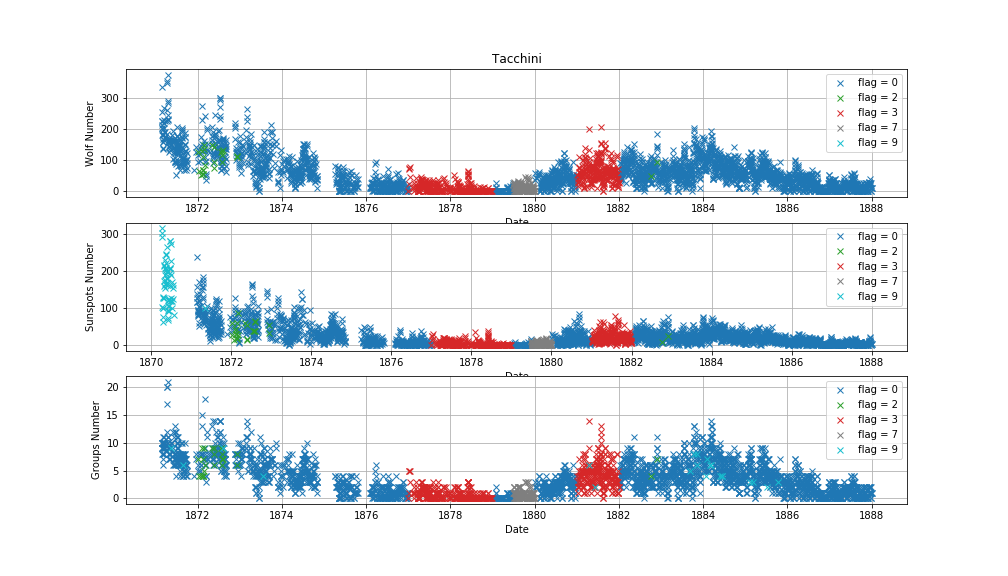
\includegraphics[width=\linewidth]{tacchini_pached.png}
\label{fig:tacchini display seperate flags all}
\par}

\subsubsection{\texttt{display\_seperate\_flags}}
This is the sister method of \texttt{display\_separate\_flags\_all} which takes an extra argument \textit{yaxis} either `sunspots', `wolf' or `groups'.  using \texttt{display\_seperate\_flags\_all}.

{\centering
\caption{Tacchini 1876-83, Sunspots only}
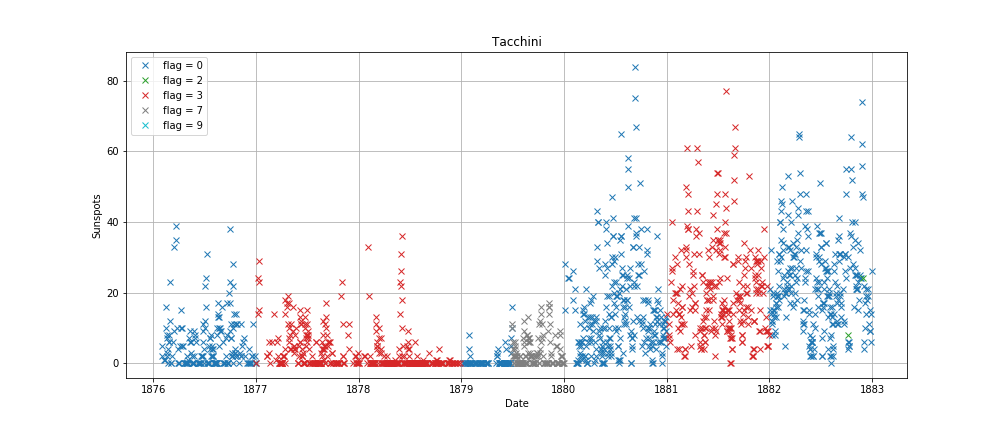
\includegraphics[width=\linewidth]{Tacchini_patches.png}
\label{fig:tacchini display seperate flags sunspots}
\par}

\subsubsection{\texttt{display\_compare\_observers}}
This method displays a scatter plot. It is very similar to \texttt{display\_seperate\_flags} but the colours represent observers rather than flags. It requires a list of observer aliases. Optionally it takes a database name \textit{the\_database} ; an \textit{interval} ; a \textit{save\_as} argument ; a \textif{figsize} argument = 2 int tuple ; an \textit{include\_flags} argument - a list of flags to display, default value is (None,0,1,2,3,4,5,6,7,8,9) ; (see \ref{fig:carrington, kew, leppig, jenzer after fix} for a demonstration of this type of plot)



\subsubsection{\texttt{display\_wolf\_drift}}
Scatter plot of the wolf number of an observer o (in blue), and a plot of $\frac{w_o - w_a}{w_a + 10}$ vs date. $w_o$ is the wolf number of the observer, $w_a$ is the accepted wolf value of the sunspot number series $v 2.0$. The idea here was to detect a drift, if a particular observer was drifting was progressively seeing less and less spots (because of declining eyesight or some other reason) and assuming $v 2.0$ of the sunspots number series is correct, this plot would expose the trend. Unfortunately (or fortunately depending on which way you look at it) I was not able to detect a drift in any of the observers I plotted with this. \\

{\centering
\caption{}
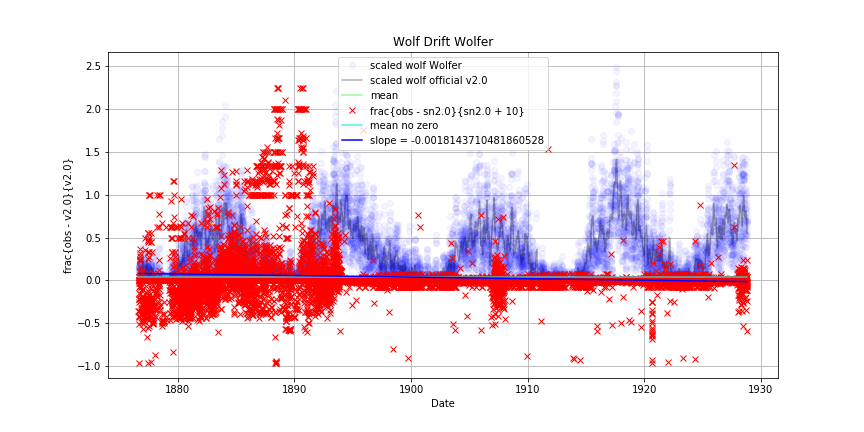
\includegraphics[width=\linewidth]{wolfer_drift.png}
\label{}
\par}



\subsection{Histogram}
\subsubsection{\texttt{frequency\_wolf\_histogram}}
Takes a single observer alias : String - \textit{observer} and plots a histogram wolf/sunspots/groups number (x-axis) vs number of times each value was observed (y-axis). Optionally it takes : \\
2 String tuples - an \textit{interval} - (`yyyy-mm-dd',`yyyy-mm-dd') ;\\
2 int tuple - \textit{figsize} - (18,14) ; \\
String - \textit{save\_as} if specified saves the figure as image - `Tacchini\_histogram.png' ; \\
String - \textit{option} - `wolf'/`sunspots'/`groups' ; \\
boolean - \textit{zero} - if False the zero measurements are left out ; \\
int \textit{binwidth} ; \\
boolean - \textit{only\_blue} - if True only displays histogram with binwidth=1 ; \\
float - \textit{sup\_freq} - if specified, it will set a maximum for the number of observations displayed on the histogram ;\\
2 String tuple - \textit{data\_interval} - (`yyyy-mm-dd',`yyyy-mm-dd')

{\centering
\caption{}
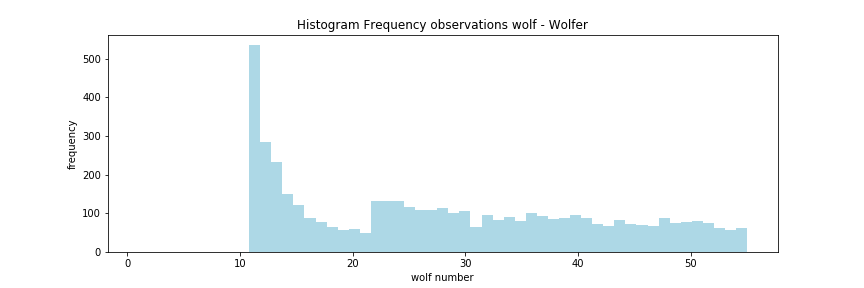
\includegraphics[width=\linewidth]{histogram_wolfer.png}
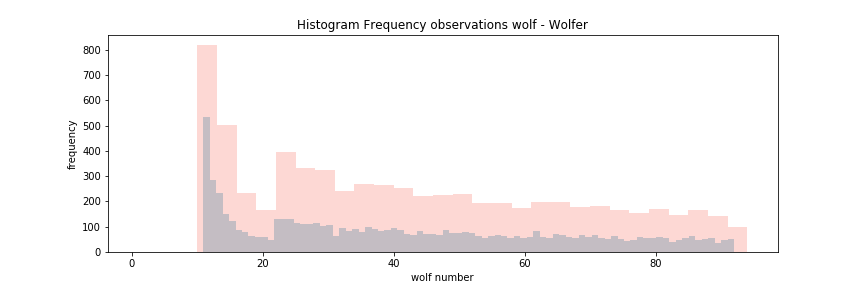
\includegraphics[width=\linewidth]{histogram_wolfer2.png}
\label{}
\par}


\subsection{Bar charts and pie charts}

See section (\ref{section:modifications made}) for the pie charts and bar charts

\subsection{Other plots}
\subsubsection{\texttt{event\_plot}}
A plot to identify when which observers are observer. Takes 2 parameters\\
2 String tuple - \textit{interval} - (`yyyy-mm-dd',`yyyy-mm-dd')\\
array like Strings - \textit{observer\_aliases} - [`obsalias1',`obsalias2']\\
Optionally takes \textit{figsize} ; \textit{fontsize} ; \textit{gridlines} ; \textit{title} ; \textit{save\_as}\\

{\centering
\cation{Two event-plots of Wolf's data : before and after}
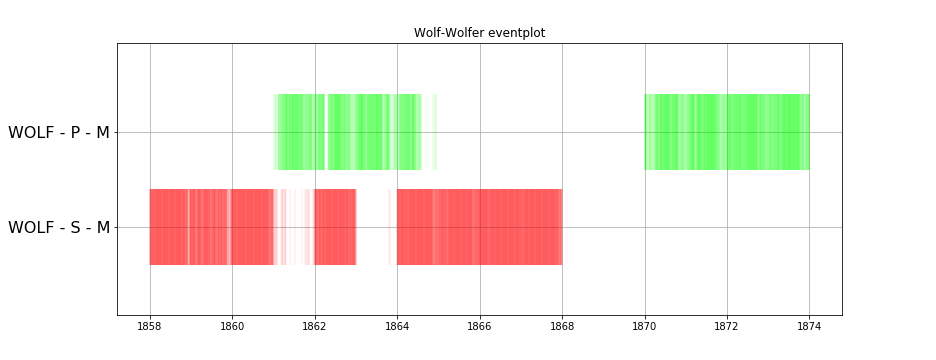
\includegraphics[width=\linewidth]{wolfSP_58_74_before.png}
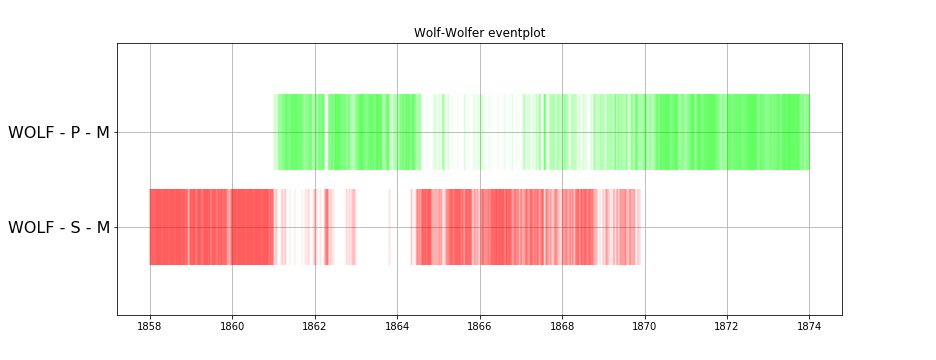
\includegraphics[width=\linewidth]{wolfSP_58_74_after.png}
\label{fig:event plots wolf before and after}
\par}

\subsubsection{\texttt{stacked\_area\_plot}}
The stacked area plots are similar to the even-plot in that they show how much an observer has been observing and when. The y axis is the frequency of observation, smoothed (otherwise it's just 1's and 0's), the x axis is the date. The method takes \\
2 String tuple - \textit{interval} - (`yyyy-mm-dd',`yyyy-mm-dd') ;\\
2 int tuple - \textit{figsize} ;\\
String -  \textit{save\_as} ;\\
float or int - \textit{smootheness} ;\\
array like String - \textit{observers\_list} ; \\
boolean - \textit{display\_others} ; \\
boolean - \textit{display\_legend} ;\\
String - \textit{plot\_title} ;\\

{\centering
\caption{Stacked area chart Wolf, Wolfer, schwabe + some others}
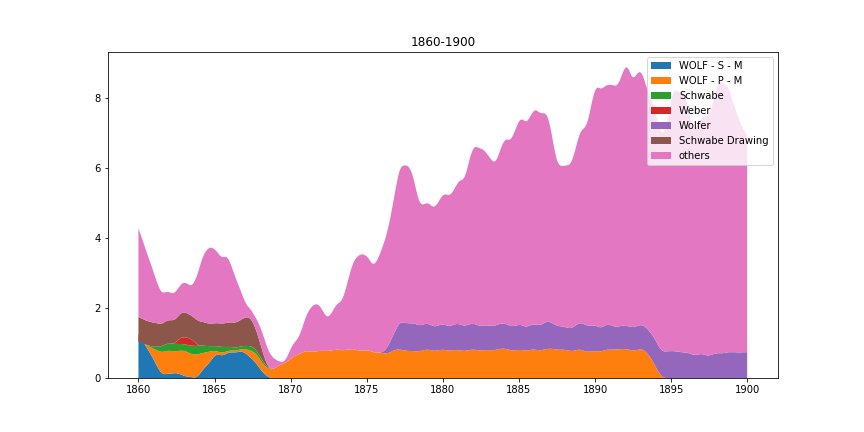
\includegraphics[width=\linewidth]{stacked_wolf_wolfer_schwabe.png}
\label{fig:stacked wolf wolfer schwabe}
\par}\\




\section{Condensed Log}

\subsection{Before The Solstice}
Started the log on the $21^{st}$. Up till now I've been learning the basics of \texttt{SQL} and how to interface with an \texttt{SQL} database through the mysql terminal; acquainting myself with the data and with what it is I ought to be doing. This is the period where I wrote some of the basic methods for accessing and connecting with the Mittheilungen database.

\subsection{Friday June 21}
\begin{itemize}
    \item Started writing the log
    \item Made `searching\_the\_manuals.py'
    \item Searching database for `uncertain' comments
\end{itemize}
    
\subsection{Monday June 24}
\begin{itemize}
    \item Discovered and sorted many duplicated data-points, (duplicate means two dta-pts for one date and one observer)
    \item Methods used can be found in \texttt{searching\_the\_manuals.py}
\end{itemize}
    
\subsection{Tuesday June 25}
\begin{itemize}
    \item Backed up the databases and started flagging for the moving process.
    \item Wrote a new script to deal uniquely with deleting the duplicates (and putting them into `\texttt{RUBBISH\_DATA}')
    \item Commented the rubbished duplicate data points
\end{itemize}
    
\subsection{Wednesday June 26}
\begin{itemize}
    \item Wrote methods for finer mass commenting (in \texttt{db\_edit.py})
    \item Flagged data with abnormally large groups and or sunspots numbers.
    \item Set 212 flags 3 for putting things in the bin. There are still 4000 pairs of duplicates that need attending to, originally there where 14000
\end{itemize}
    
\subsection{Thursday June 27}
\begin{itemize}
    \item Moved the flagged duplicates to \texttt{RUBBISH\_DATA}
    \item Found entire rubrics worth of data written in wrong year
    \item Started writing \texttt{corrections\_needed\_handwritten.txt}, to make clear all my tasks.
\end{itemize}
    
\subsection{Friday June 28} 
\begin{itemize}
    \item The notes I took about the duplicates can be found in different\_value\_duplicates.txt, some things I found interesting so I decided to copy most of the file into this report (see long version of the log)
\end{itemize}
    
\subsection{Monday July 1}
\begin{itemize}
    \item Using what I did on Friday to bin some duplicated data and modify some other data
    \item Made a new alias in \texttt{DATA\_SILSO\_HISTO} (and \texttt{BAD\_DATA\_SILSO}) called `Brunner Assistent'.
\end{itemize}
    
\subsection{Tuesday July 2}
\begin{itemize}
    \item Made some pretty plots in \textit{suspicious sunspots plots.ipynb} in the root directory
    \item Made a method in the jupyter notebook mentioned above that plots an observer's data and color codes the flags.
    \item Started patching Tacchini's missing holes
\end{itemize}
    
\subsection{Wednesday July 3}\label{what is flag 2 question mark}
\begin{itemize}
    \item Continued fixing Tacchini (see figure \ref{fig:tacchini})
    \item Went back to searching the manuals for errors from error sheet. Looking for `uncertain' comments.
    \item Figured out what COMMENT=`?' means! It means blurry image, or bad definition of img
    \item Found some comments where there is both an observer and a question mark at the same time, for these ones I left the comments as they are and changed only the flag from 1 to 2.
    \item Finished looking at red comments (I still need to change them and move them all with python, I will do it tomorrow.)
    \end{itemize}
            
\subsection{Thursday July 4}
\begin{itemize}
    \item Looking into Carrington's case.
    \item I updated the flag 7 to ``derived from area-measurement" and flagged all of Secchi's sunspot values that were derived from the penumbra and / or umbra.
    \item Spoke to F. Clette about the possible conversion from the `aire' to a sunspots number. He gave me some clues as to where to look in the mitt.
    \item Excitement! I found on page 131 of Mitt 31-40 written after rubrics 299 a description of how the author (I think R. Wolf himself) derived a formula for turning Secchi's `aire' into a sunspots number (the rubrics is translated in the log)
\end{itemize}
        
\subsection{Friday July 5}
\begin{itemize}
    \item Continued working on Carrington - Main event = did a least-squares regression fit to optimise the constant values in the equation that transforms `aire' into wolf number.
\end{itemize}

\subsection{Monday July 8}
\begin{itemize}
    \item Finished deriving Carrington
    \item Backed up databases
\end{itemize}

\subsection{Tuesday July 9}
\begin{itemize}
    \item Derived Kew's misbehaving data
    \item Made a new `README.md' that auto-generates based on what is inside my python scripts
    \item Tidied the report and added some figures
\end{itemize}

\subsection{Wednesday July 10}
\begin{itemize}
    \item Separated Carrington into two aliases
    \item Figured out what to do with Secchi (now I just have to do it)
\end{itemize}

\subsection{Thursday July 11}
\begin{itemize}
    \item Dealt with rubrics 375, see \texttt{secchi\_derivation.ipynb}
    \item Dealt with 2 more of Secchi's rubrics, there are still 2 annoying ones
    \item Continued checking and correcting typos and anomalies from the blue comments sheet
\end{itemize}

\subsection{Friday July 12}
\begin{itemize}
    \item Dealt with the red comments, changed alot of their comment to `?' which was written in the journals and changed the flag to 2
    \item Put some thought into how to deal with oranges aswell as Wolf / Wolfer
\end{itemize}

\subsection{Monday July 15}
\begin{itemize}
    \item Transferred all the data with flag = 2 into the database \texttt{GOOD\_DATA\_SILSO}
    \item Upgraded the plotting methods in \texttt{graphs\_helper.py} and plotted Wolf and Wolfer and aliases in which they appear - see \texttt{wolf\_wolfer\_investigation.ipynb}
    \item Brainstormed how I was gonna tackle wolf / wolfer's data
\end{itemize}

\subsection{Tuesday July 16}
\begin{itemize}
    \item Wrote some methods to smooth data and also to plot the sunspots number
    \item Corrected typos and errors
\end{itemize}

\subsection{Wednesday July 17}
\begin{itemize}
    \item Corrected Adam's data by hand data-point by data-point
    \item Made some more plots in the \texttt{wolf\_wolfer\_investigation.ipynb}
    \item Accidentally deleted database and lost all the edits I made to the database today... :(  [luckily I have backups from yesterday]
\end{itemize}

\subsection{Thursday July 18}
\begin{itemize}
    \item Accidentally deleted the data again, re-corrected Adam's data manually
    \item Fixed the data and imported the old data into the database \texttt{ORIGINAL\_DATA\_SILSO\_HISTO}
    \item Wrote to Laure and she gave me some good ideas for how to detect drift
    \item Rereading papers to get better understanding of what I ought to be doing
\end{itemize}

\subsection{Friday July 19}
\begin{itemize}
    \item Made a plotting tool in an attempt to visualise the drift of observers, unfortunately it didn't work out brilliantly (it's not very helpful)
    \item Made a couple new aliases which I populated with data `Mooser' (for rubrics 122 only)
    \item Made the alias `Wolfer P' who now has 307 data-points.
\end{itemize}

\subsection{Monday July 22}
\begin{itemize}
    \item Wrote a cute little script to automate backing up the databases and committing with git (there will be more frequent backups now).
    \item Translated a long rubric
    \item Sorted all the data attached to fk\_observers IN (60,61,62) - all composite observers from these strange rubrics\_number = 0 in the mid to late 1800's - into their proper observers.
\end{itemize}

\subsection{Tuesday July 23}
\begin{itemize}
    \item Made some fancy plots and plotting tools : \texttt{size\_data\_by\_observers()} plots a bar chart of of all the observer aliases on the x axis and on the y axis it plots how many data-points are associated with them ; \texttt{event\_plots()} shows you the observer aliases on the y axis this time, and the x axis is the dates, plotted is all the dates each one observed on.
\end{itemize}

\subsection{Wednesday July 24}
\begin{itemize}
    \item Updated the \texttt{create\_readme.py} file
    \item Did some event plots and investigated `Ricco, Zona, Mascari'
    \item Learned a whole lot of things from F. Clette about his work, the current state of solar physics and some interesting things about Burnner and other observers
\end{itemize}

\subsection{Thursday July 25}
\begin{itemize}
    \item Re-plotted some data from the Wolf - Wolfer transition period that has been modified since last time I plotted it and the change is magnificent! 
    \item Finally abolished `Ricco, Zona, Mascari' and appropriately sorted the data
    \item Launched an investigation of rubrics 684 which is very confusing. There are many problems with it.
\end{itemize}

\subsection{Friday July 26}
\begin{itemize}
    \item Sorted out rubrics 684 (Kremsmunster)
\end{itemize}

\subsection{Monday July 29}
\begin{itemize}
    \item Started investigating Wolf and Schwabe's mysterious holes
\end{itemize}

\subsection{Tuesday July 30}
\begin{itemize}
    \item Doing some archaeological excavations on the Wolf mixup and Mitteilungens 1 though 10 
    \item Deleted some erroneous data of WOLF - S - M (same needs to be done for 67)
    \item Failed to find a suitable correction for certain things see log for details
\end{itemize}

\subsection{Wednesday July 31}
\begin{itemize}
    \item Did some more corrections on Wolf's data (basically data-entry)
\end{itemize}

\subsection{Thursday August 1}
\begin{itemize}
    \item Discovery, R. Wolf uses 3 telescopes not 2. While he is in charge of the observatory in Zurich he uses what he refers to as the `$\times 64$ magnification quadruped' (paraphrasing), in 1870 he switches primary telescope to the Parisian $\times 20$ magnification, and all the while when he goes on trips he takes with him a pocket telescope. It is still unclear as to weather he uses the Parisian much before 1870, my guess is that while he was still going to the observatory every day all the official measurements would be made with the big one, and the Parisian which most likely stayed in his home was used only for recreational purposes.
\end{itemize}

\subsection{Friday August 2}
\begin{itemize}
    \item Found that R. Wolf might actually use primarily the Parisian as his secondary before his retirement (1867-9)
    \item Added Schwabe's online data to the databases
    \item Made a method to make stacked area plots for the frequency of observation
\end{itemize}

\subsection{Monday August 5}
\begin{itemize}
    \item Perfected stacked area plots to point of being fully functional with options
    \item Started having a go at the orange highlighted comments - am changing aliases based off of comments, after cross checking what the comment says and what is written in the preamble of the rubric each time of course.
\end{itemize}

\subsection{Tuesday August 6}
\begin{itemize}
    \item Cleared out some of the data in BAD DATA SILSO which was flagged weirdly (lots of the data points with flag = 4)
    \item Found some of Wolf's missing data
\end{itemize}

\subsection{Wednesday August 7}
\begin{itemize}
    \item Thoroughly scrutinized Wolf's data in the Mittheilungen journals and arranged my findings into a table with crucial information concerning his observations
\end{itemize}

\subsection{Thursday August 8}
\begin{itemize}
    \item Did some final updates of the data flagged with flag=4, flag=5 and flag=9
    \item Corrected `Schwabe Drawing' 's data
    \item Made some edits to the flag section of the report
\end{itemize}

\subsection{Friday August 9}
\begin{itemize}
    \item Made the histogram plotting methods
\end{itemize}

\subsection{Monday August 12}
\begin{itemize}
    \item Plotted the pie-charts and bar-charts that display the changes that I have effectuated to the database.
    \item Brainstormed final draft of report
\end{itemize}

\subsection{Tuesday August 13}
\begin{itemize}
    \item Modified some of the plotting functions
    \item Started writing second draft of report
\end{itemize}



\section{Conclusions and Ideas for Future Work}
Though the quality of the data has been improved it is not yet perfect. There are still some crucial modifications to be made. Some of these require the Mittheilungen journals, I am thinking specifically of those with flag = 1 where a secondary observer is commented. The data flagged 0 is reliable according to my (unprofessional) assessment. I have separated the troublesome data into 8 categories (8 flags) so that it is easier to understand what is wrong with it, my hope is that these can be used in limited ways rather than not at all - or that they are used irresponsibly in situations where they are invalid. 

\subsection{Ideas for the detection of new errors}
\begin{itemize}
\item Though this was done to some degree, a more thorough job can be made of using the plotting functions I developed to detect errors. The event-plot can be used to detect errors similar to the Wolf / Wolfer outliers that were detected with the event-plot. What I have in mind is to do event-plots of each of the observers.
\item A script to detect isolated data-points : for each observer's data-set, find data-points that are very far-out. 
\item A script for the detection of data-points in the wrong year : for each rubric find the data-points that are in a year that is not the norm, so if there is like $<1\%$ of your data is in a year different than the rest...
\end{itemize}

\section{Miscellaneous}

\subsection{SQL data-table format}

\subsubsection{SQL data tables format 1 - original format}

%\begin{table}[h!]
{\centering
    \caption{\texttt{DESCRIBE DATA}}
    \begin{tabular}{c|c|c|c|c|c}% l c r = Left Centre Right
        \textbf{Field} & \textbf{Type} & \textbf{Null} & \textbf{Key} & \textbf{Default} & \textbf{Extra}  \\
        \hline
        ID & int(11) & No & PRI & NULL & auto\_increment \\
        
        DATE & date & YES && NULL & \\
        
        FK\_RUBRICS & int(11) & YES & MUL & NULL &  \\
        
        FK\_OBSERVERS & int(11) & YES & MUL & NULL &  \\
        
        GROUPS & int(11) & YES && NULL &  \\
        
        SUNSPOTS & int(11) & YES && NULL & \\
        
        WOLF & int(11) & YES && NULL &  \\
        
        QUALITY & int(11) & YES && NULL &  \\
        
        COMMENT & text & YES && NULL &  \\
        
        DATE\_INSERT & datetime & YES && NULL &  \\
        
        FLAG (i added this) & tinyint(1) & YES && NULL &  \\
        
    \end{tabular}
    \label{tab:data-og}
\par}\\
%\end{table}

%\begin{table}[h!]
{\centering
    \caption{\texttt{DESCRIBE OBSERVERS}}
    \begin{tabular}{c|c|c|c|c|c}% l c r = Left Centre Right
        \textbf{Field} & \textbf{Type} & \textbf{Null} & \textbf{Key} & \textbf{Default} & \textbf{Extra}  \\
        \hline
        ID & int(11) & NO & PRI & NULL & auto\_increment \\
        
        ALIAS & varchar(50) & YES && NULL & \\
        
        FIRST\_NAME & varchar(50) & YES && NULL &  \\
        
        LAST\_NAME & varchar(50) & YES && NULL &  \\
        
        COUNTRY & varchar(50) & YES && NULL &  \\
        
        INSTRUMENT & varchar(50) & YES && NULL & \\
        
        COMMENT & text & YES && NULL &  \\
        
        DATE\_INSERT & datetime & YES && NULL &  \\
        
    \end{tabular}
    \label{tab:data-og}
\par}\\
%\end{table}

%\begin{table}[h!]
{\centering
    \caption{\texttt{DESCRIBE RUBRICS}}
    \begin{tabular}{c|c|c|c|c|c}% l c r = Left Centre Right
        \textbf{Field} & \textbf{Type} & \textbf{Null} & \textbf{Key} & \textbf{Default} & \textbf{Extra}  \\
        \hline
        RUBRICS\_ID & int(11) & NO & PRI & NULL & auto\_increment \\
        
        RUBRICS\_NUMBER & int(11) unsigned & NO && NULL & \\
        
        MITT\_NUMBER & int(11) unsigned & NO && 0 &  \\
        
        PAGE\_NUMBER & int(11) unsigned & YES && NULL &  \\
        
        SOURCE & text & NO && NULL &  \\
        
        SOURCE\_DATE & date & YES && NULL & \\
        
        COMMENTS & text & YES && NULL &  \\
        
        DATE\_INSERT & datetime & YES && NULL &  \\
        
        NB\_OBS & int(11) & YES && NULL & \\
        
    \end{tabular}
    \label{tab:data-og}
\par}\\
%\end{table}

%\newpage{}

\subsubsection{SQL data table format 2}

%\begin{table}[h!]

{\centering
    \caption{\texttt{DESCRIBE DATA} (the only table)}
    \begin{tabular}{c|c|c|c|c|c}% l c r = Left Centre Right
        \textbf{Field} & \textbf{Type} & \textbf{Null} & \textbf{Key} & \textbf{Default} & \textbf{Extra}  \\
        \hline
        ID & int(11) unsigned & No & PRI & NULL & auto\_increment \\
        
        DATE & date & YES && NULL & \\
        
        GROUPS & int(11) & YES && NULL &  \\
        
        SUNSPOTS & int(11) & YES && NULL & \\
        
        WOLF & int(11) & YES && NULL &  \\
        
        COMMENT & text & YES && NULL &  \\
        
        DATE\_INSERT & datetime & YES && NULL &  \\
        
        OBS\_ALIAS & varchar(50) & YES && NULL & \\
        
        FIRST\_NAME & varchar(50) & YES && NULL & \\
        
        LAST\_NAME & varchar(50) & YES && NULL & \\
        
        COUNTRY & varchar(50) & YES && NULL & \\
        
        INSTRUMENT\_NAME & varchar(50) & YES && NULL & \\
        
        RUBRICS\_NUMBER & int(11) & YES && NULL & \\
        
        MITT\_NUMBER & int(11) & YES && NULL & \\
        
        PAGE\_NUMBER & int(11) & YES && NULL & \\
        
        FLAG & tinyint(1) unsigned & YES && NULL &  \\
        
        RUBRICS\_SOURCE & text & YES && NULL & \\
        
        RUBRICS\_SOURCE\_DATE & date & YES && NULL & \\
        
    \end{tabular}
    \label{tab:data-og}
\par}
%\end{table}

\subsection{Backbone observers table}

{\centering
\begin{tabular}{c|c|c|c}\label{table:backbone}
     Backbone Observer & Main interval & Full interval & Nb Observers  \\
     \hline
     Staudach & 1749 - 1787 & 1740 - 1822 & 15 \\
     Schwabe & 1826 - 1867 & 1794 - 1883 & 20 \\
     Wolfer & 1878 - 1928 & 1841 - 1944 & 21 \\
     Koyama & 1947 - 1993 & 1920 - 1996 & 36 \\
     Locarno & 1957 - 2015 & 1950 - 2015 & 22 \\
\end{tabular}
\par}
\footnotesize{Source : \href{https://files.aas.org/astronomy2015/Presentations/DE_Fr\%C3\%A9d\%C3\%A9ric_Clette_Heliosphere.pdf}{https://files.aas.org/astronomy2015/Presentations/DE_Fr\%C3\%A9d\%C3\%A9ric_Clette_Heliosphere.pdf}}

\subsection{Ideas for the detection of more problems that never saw the light of day}
\subsubsection{Detecting rubrics-wide typos}
In the duplicates section (\ref{section:duplicated data}) there were entire rubrics entered in the wrong year / under the wrong observer. The only reason they were detected by the duplicates finding algorithms was because they just so happened to be entered into a year where there was already data for that same observer, or in the case of the wrong observer, they were written in under an observer who was also observing in at the same time. It is possible that some data was entered in the wrong year / under the wrong observer without coinciding with other data and so went undetected by these methods.\\

\subsubsection{Estimating the number of typo-like errors with sample}
This section here is probably useless and I will delete it if anyone gives the word but I just couldn't help myself\\

If we sample $n$ data points from our database of $N \approx 205 000$, for each of the $n$ sampled we check in the Mittheilungen to see if the data-point is correctly entered and we find that $k$ of the $n$ have problems. Given the probability that any given data-point is erroneous is $p$. We denote the probability of obtaining $k$ given $n$ and $p$ by $\lambda$. \\

\begin{equation}
    \lambda(n,k,p) = {n \choose k} p^k (1-p)^{n-k}
\end{equation}

Then we can estimate the probability of a data-point being troublesome $p_0$. 

\begin{equation}
    \frac{d\lambda}{dp} = 0 = {n \choose k} p_0^{k-1} (1-p_0)^{n-k-1} \cdot (k-np_0)
    , \quad p_0 \in (0,1) \quad \RA \quad 
    p_0 = \frac{k}{n}
\end{equation}

And estimate a standard deviation $\sigma$ with equation \ref{equation:std of integral of lambda} that tells us how close our term $p_0$ is likely to be close to the truth. Assuming the polynomial function looks roughly gaussian around $p_0$. This should be easy to do analytically (with a computer) since $\lambda$ is a polynomial.

\begin{equation}\label{equation:std of integral of lambda}
    \int_{p_0-\sigma}^{p_0+\sigma} \lambda(n,k,p) dp = 0.6827 \cdot \int_0^1 \lambda(n,k,p) dp
\end{equation}

Which it does, here I plotted $\lambda$ with the values $k=21$ and $n=1000$ (I didn't normalise the area that's why it's so small). I wonder if the function converges locally onto a gaussian at the limit $n\to\inf$, I guess they must because they both become the dirac delta... But it's funny that the gaussian pops up here because the poisson we were using for the binomial distribution for the discrete probability.\\

{\centering
\caption{}
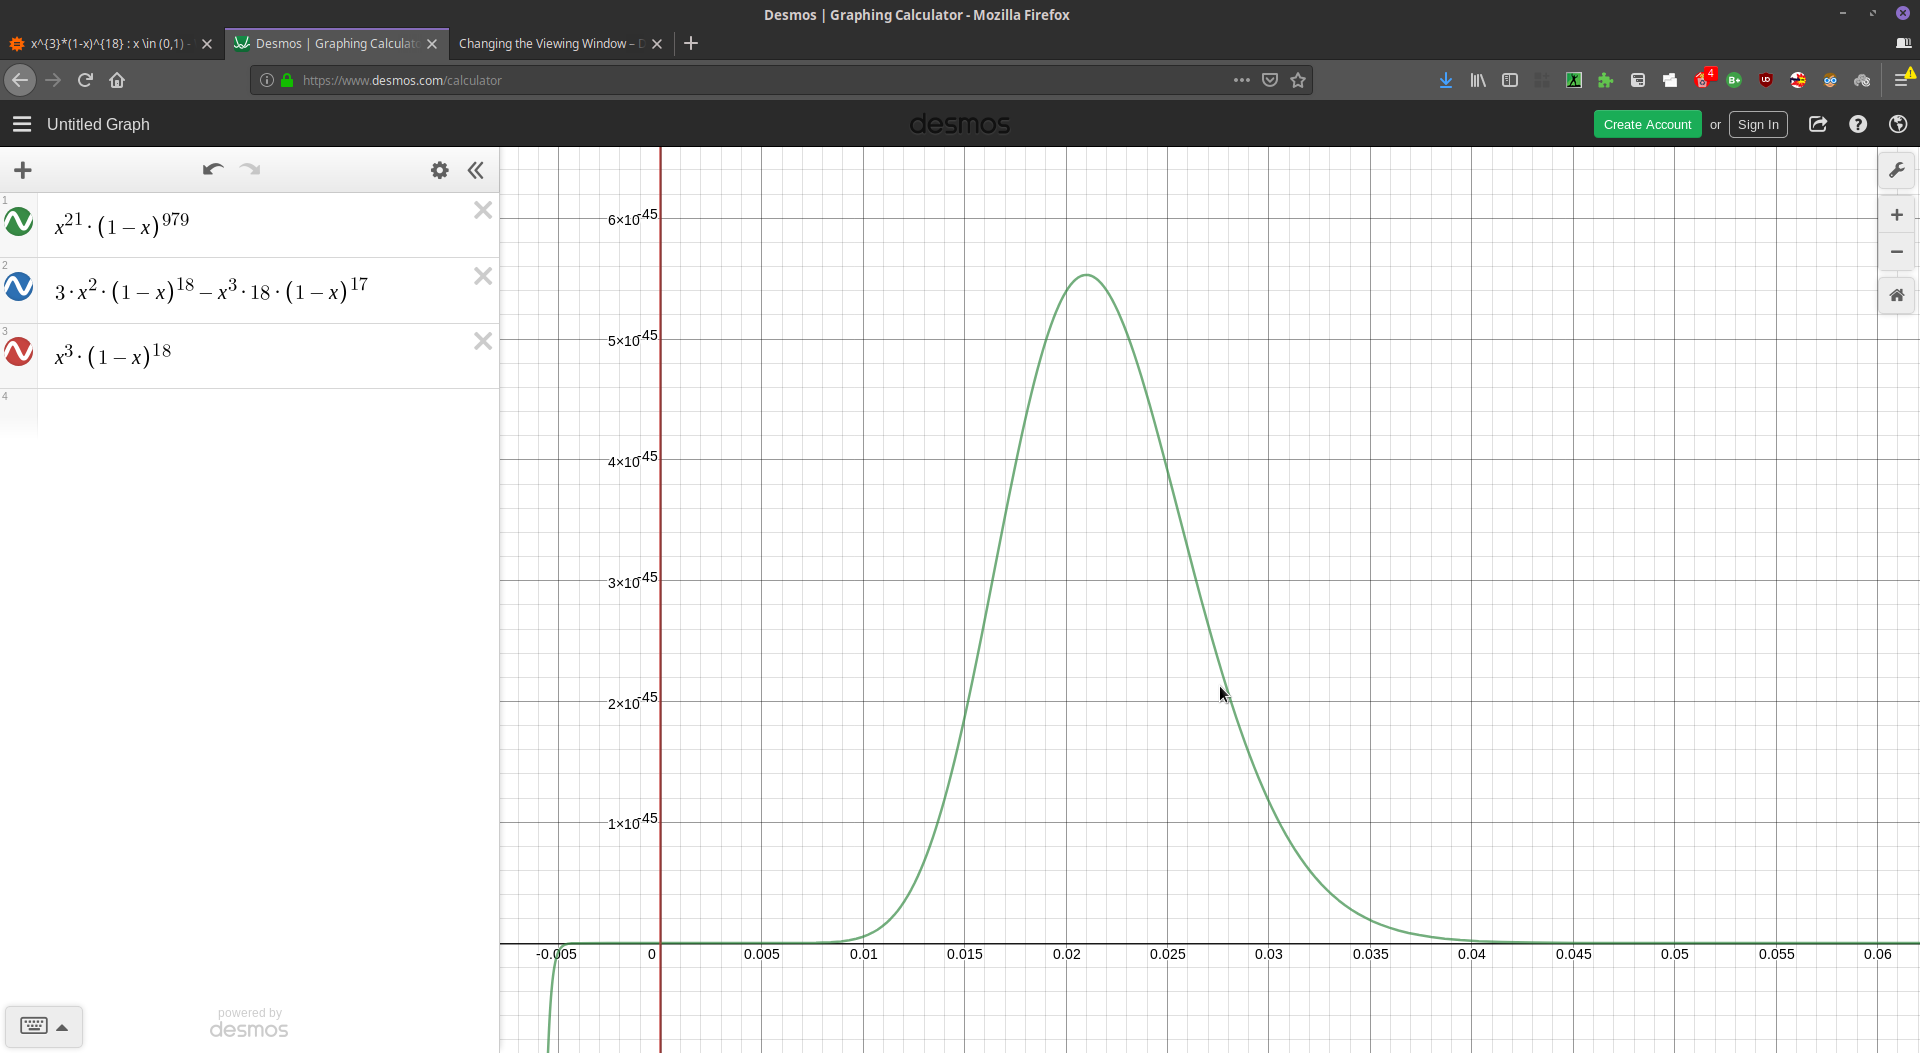
\includegraphics[width=\linewidth]{Screenshot at 2019-08-19 00-20-14.png}
\par}


\subsection{Notes}
\begin{itemize}
    \item There are 3 different Sykora's : Herr N. Sykora (aka Sykora-N) ; Fraulein O. Sykora (aka Sykora-O-67mm) ; J. Sykora (aka Sykora)\label{section:info sykora}
    \item William Otto Brunner's assistent may be several different people : his wife Hagger ; his nephew.
\end{itemize}



\end{document}

